\section{Experimental Method (SV, KF, BB)}

This section fully explains the processes undertaken in order to complete this project. It includes  information regarding personnel involved, expenditures undertaken and relevant venues, as well as a full, detailed list of equipment used.

\subsection{Equipment list}

In its final iteration the experimental apparatus...\todo{Apparatus description}

Below is a full list of equipment used in various stages of the experiment. More information about how each piece of equipment is utilised is included in the following sections.
\bigskip
\begin{enumerate}

\item \textbf{Speaker: QXW6 6.5'' High Power Woofer with Kevlar Cone - QTX \ref{fig:speaker}:}

\begin{itemize}
\item 250W power max
\item 8$\Omega$ impedance
\item 1.92kg
\item 88.0dB
\item Frequency Response: 35Hz - 8kHz
\item Overall depth: 90mm; Diameter: 16.5cm
\end{itemize}
\item \textbf{Liquids:}

\begin{itemize}
\item 1000 cSt silicone Oil - From Derreck
\item 50 cSt silicone Oil - Alfa Aesar, 63148-62-9, L05379
\item Fairy Liquid washing up liquid
\item Water
\item Sunflower oil - Sainsbury's
\end{itemize}
\item \textbf{Recording Equipment:}

\begin{itemize}
\item Photron Fastcam SA1.1 Type 675K M1 \ref{fig:PhotronCamera}

\begin{itemize}
\item Input DC20-36V / 130VA
\item Resolution of 1024 x 1024 pixels at 5400fps
\item Maximum framerate of 675,000fps at resolution of 64 x 16
\end{itemize}
\item Lumix flash camera with GVaro 14-42 zoom lens 1:3.5 - From Kelvin Vine (Physics Film Makers)
\item Photron Spectrum Lumination P/N EL2150-WHI lighting \ref{fig:PhotronLighting}

\begin{itemize}
\item Manfrotto Photo Variable Friction Arm with Bracket, SKU 244
\end{itemize}
\item iPhone X, iOS:11.1.5 , published recorded rate: 240 fps

\item Sony Cyber-shot RX-100 IV Camera, 4K, 20.1MP, 2.9x Optical Zoom, Wi-Fi, NFC, OLED EVF, 3'' Tiltable Screen (1000fps camera)
\item Diffuser
\item High powered lighting - TriLite Max 3x30W Compact Flourescent Lamps 220-240V. Bowens, 3.15A (F)
\end{itemize}
\item \textbf{Software:}

\begin{itemize}
\item Photron FASTCAM Software - PFV Ver.3681
\item Adobe AfterEffects CS6
\item Adobe Premiere Pro CS6
\item Adobe Illustrator CS6
\item Google Sketchup
\item Sound Meter - Mobile App
\end{itemize}
\item \textbf{Machinery - Institute of Making:}

\begin{itemize}
\item Lasercutter
\item Bandsaw
\end{itemize}

\item \textbf{Signal Generators / Amplifier:}

\begin{itemize}
\item Griffin signal generator and amplifier \ref{fig:griffinsSigGen}
\item ISO-TECH Synthesized function generator GFG2004 
\item Hi-Fi amplifier ELEGIANT mini 20W 12V hi-fi car stereo amplifier LP-838 \ref{fig:amplifier}

\begin{itemize}
\item Kasstino Power Supply Adapter 12V AC 100-240V To DC 12V 2A 24W for LED Strips
\end{itemize}
\end{itemize}
\item \textbf{Miscellaneo:}

\begin{itemize}
\item Cardboard square
\item Circular plywood plate
\item 3.5'' glass petri dish - from Chemistry (2nd Floor Turner Labs, Christopher Ingold) \ref{fig:PetriDish}
\item 6'' plastic petri dish - from Chemistry (2nd Floor Turner Labs, Christopher Ingold)
\item Square tupperware box (135mm x 135mm)
\item LE LED USB Light Strip, SKU: 4100072-RGB

\begin{itemize}
\item Power: 5W
\item 16 lighting colours
\end{itemize}
\item Optical microscope
\item Soldering iron \& solder
\item Plastic strips - from plastic binder
\item Plastic pipette (1mm \& 3mm) - from Chemistry (2nd Floor Turner Labs, Christopher Ingold) chemistry lab
\item Digital Thermometer - 2000T - \ Thermometer, -200$\degree$C to +1350$\degree$C, 155 mm, 67 mm, 40 mm Type Input, Intrinsically Safe
\item Multimeter
\item 3mm Laser grade plywood
\item Red food colouring

\begin{itemize}
\item ASDA natural food colouring - red
\item Dr Oetker bright red gel food colour 15g
\end{itemize}
\item Electric cables

\begin{itemize}
\item BNC cables
\item Banana plugs (amplifier to speaker)
\item 3.5mm jack to aux (laptop to amplifier)
\end{itemize}

\item Double sided tape
\item Plastic \& glass syringe - from Andrew Redfearn
\item Spray duster - Dataflash, DF1270
\item Knitting Needle \ref{fig:DropletCreators}
\item Wood cuttings

\begin{itemize}
\item Grated cuttings - leftover from laser cutting \ref{fig:DropletCreators}
\item Solid blocks - from IoM
\end{itemize}
\item Foldback clips (clamps) - Q-Connect, 42mm
\item 1mm graph paper - Chartwell, A4-641C
\item Superglue - UHU
\item Metal ruler - 30cm
\end{itemize}
\end{enumerate}

\begin{figure}[ht]
    \begin{subfigure}{0.5\textwidth}
        \centering
        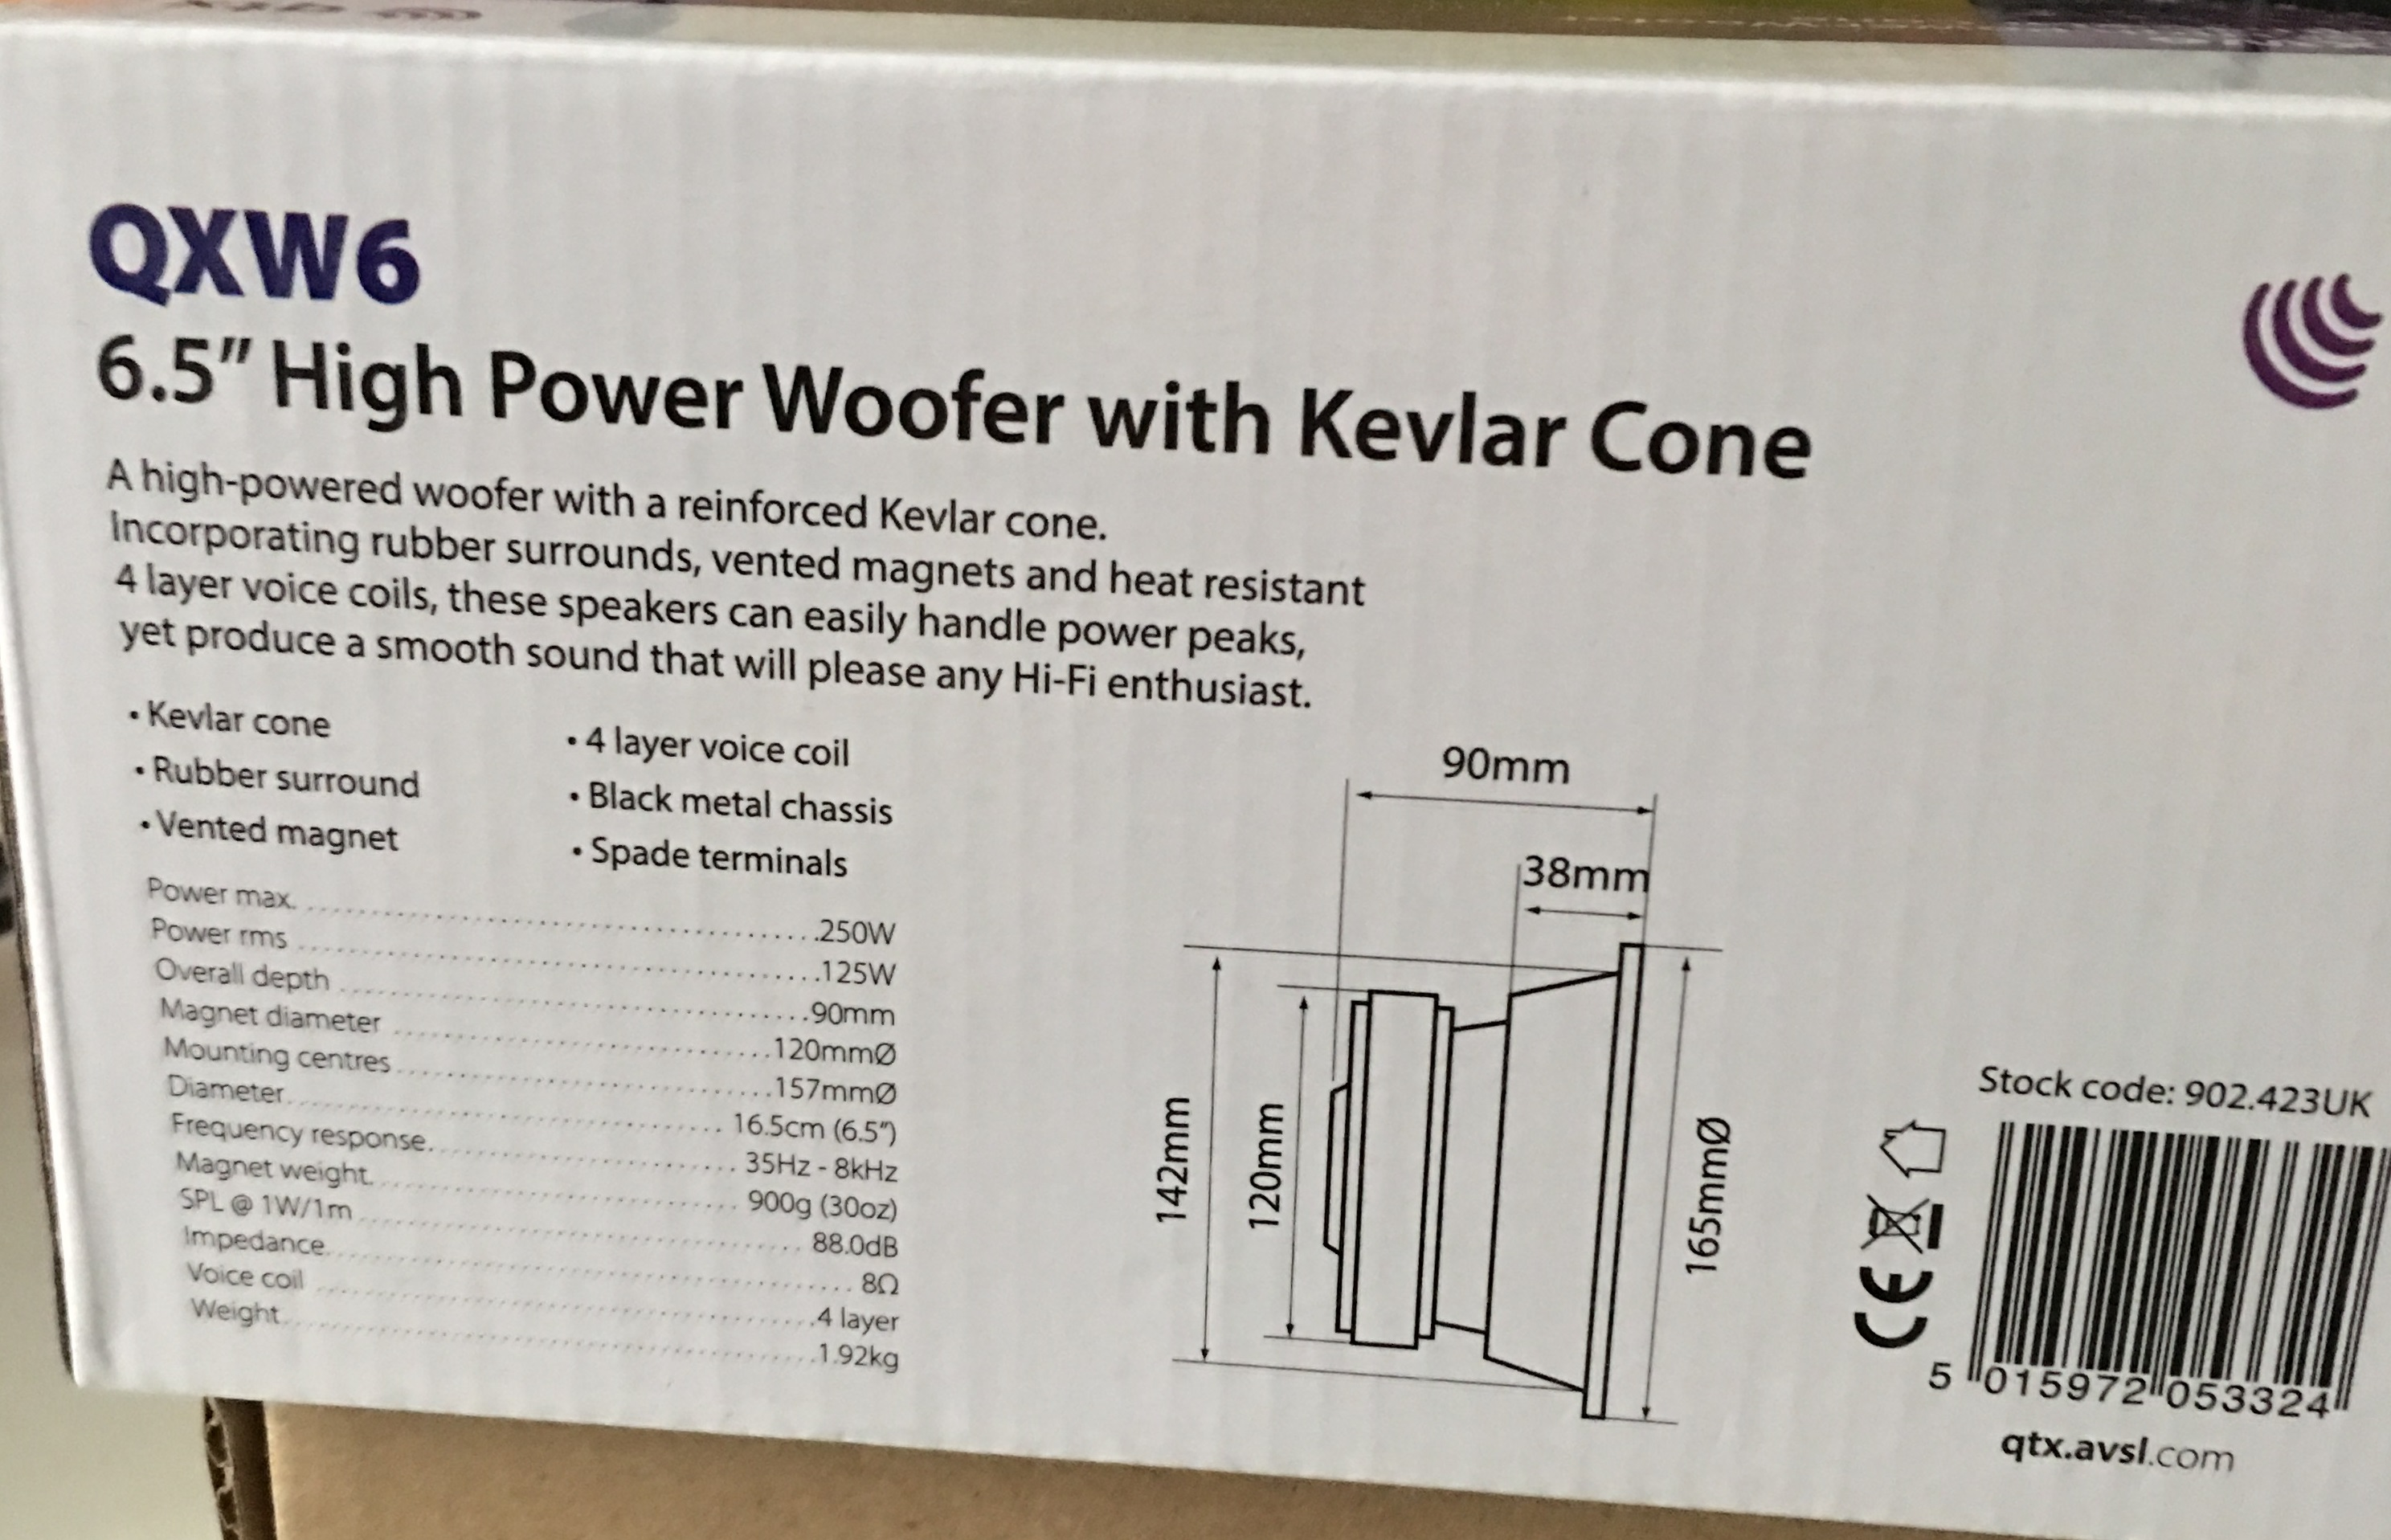
\includegraphics[width=\textwidth]{prototype/exp_rep_imgs/speakerPackaging.jpg}
        \caption{Packaging of the woofer used}
    \end{subfigure}
    \begin{subfigure}{0.5\textwidth}
        \centering
        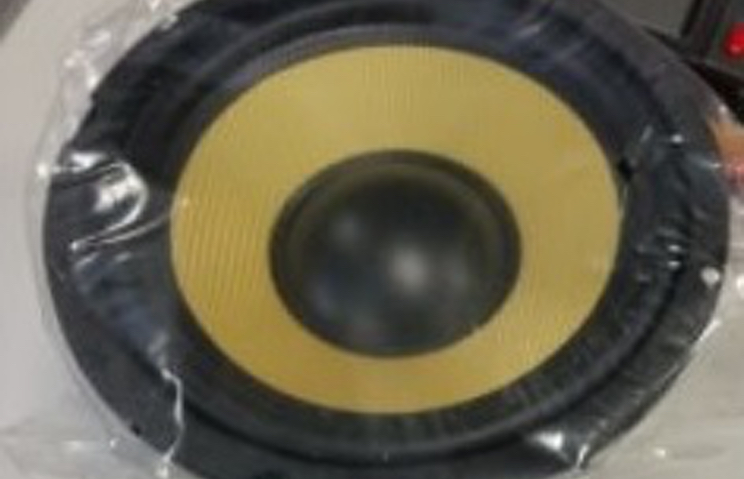
\includegraphics[width=\textwidth]{prototype/exp_rep_imgs/Speaker.jpg}
        \caption{The woofer used to carry out oscillations}
    \end{subfigure}
\caption{Images of the speaker and its packaging utilised in vibrating the liquid surface. The packaging image provides technical information regarding the woofer and its dimensions}
\label{fig:speaker}
\end{figure}

\begin{figure}[ht]
    \begin{subfigure}{0.5\textwidth}
        \centering
        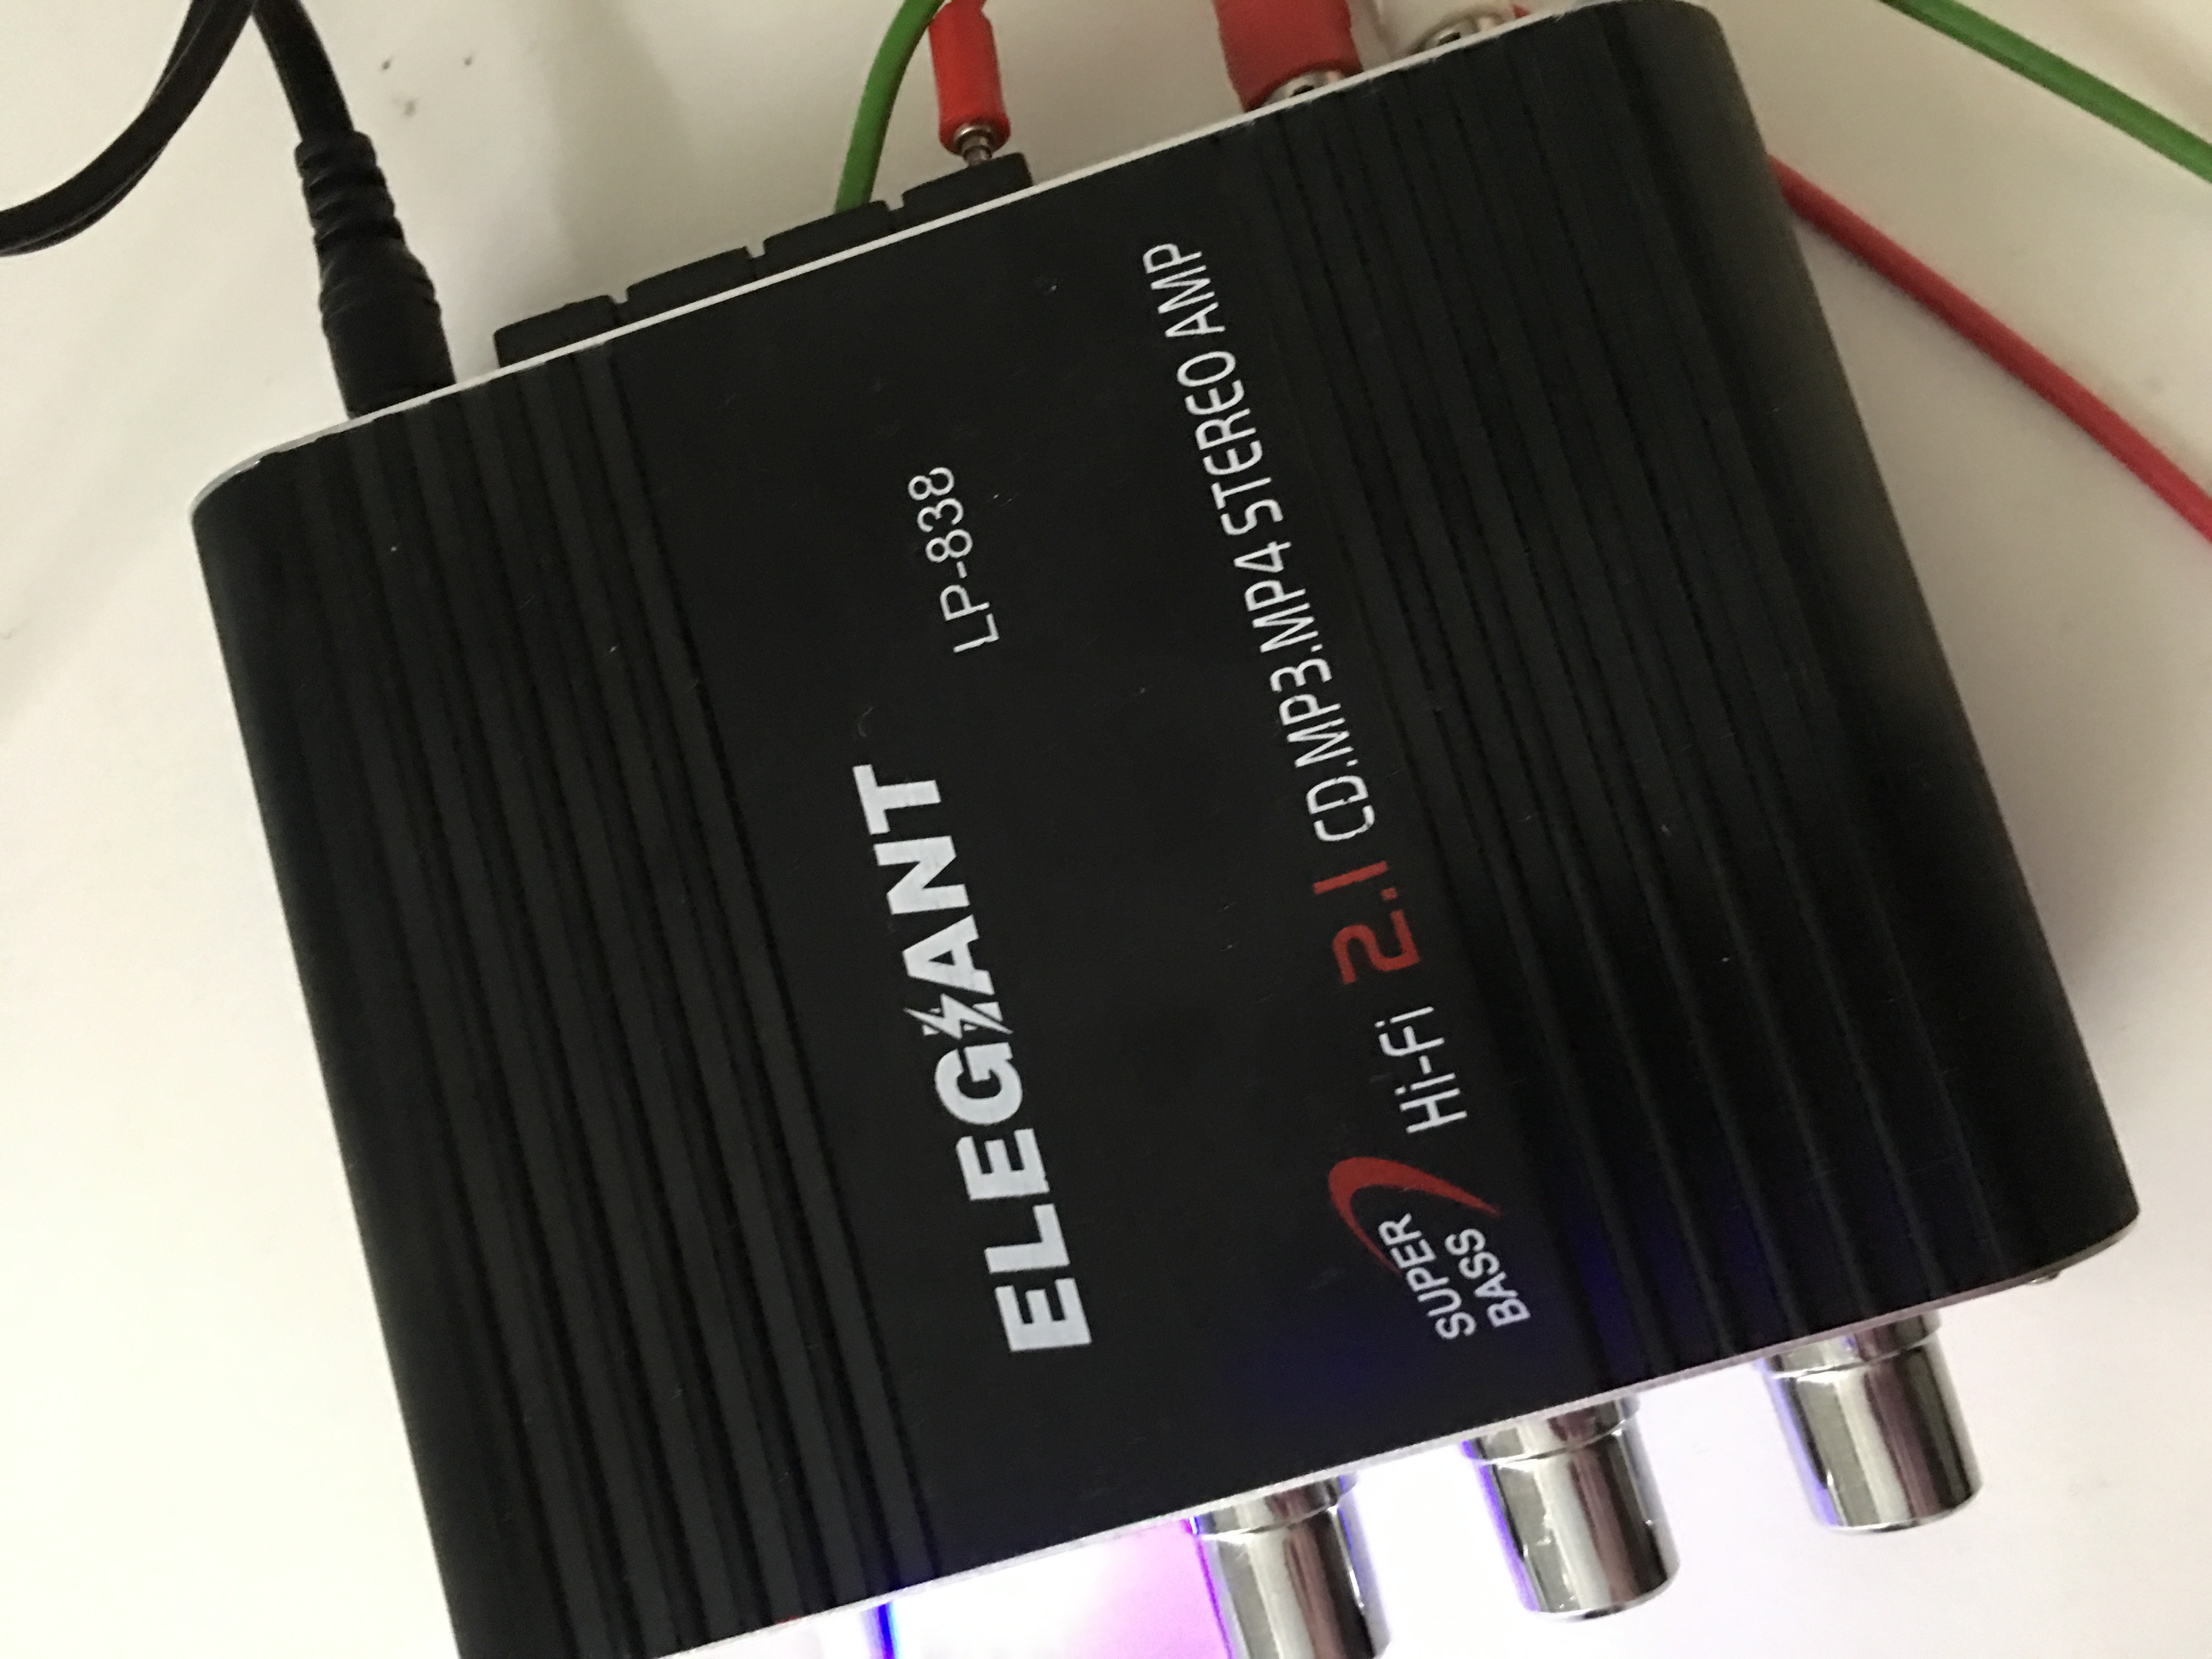
\includegraphics[width=\textwidth]{prototype/exp_rep_imgs/LEGIANT_amp.jpg}
        \caption{Top-down image of the amplifier}
    \end{subfigure}
    \begin{subfigure}{0.5\textwidth}
        \centering
        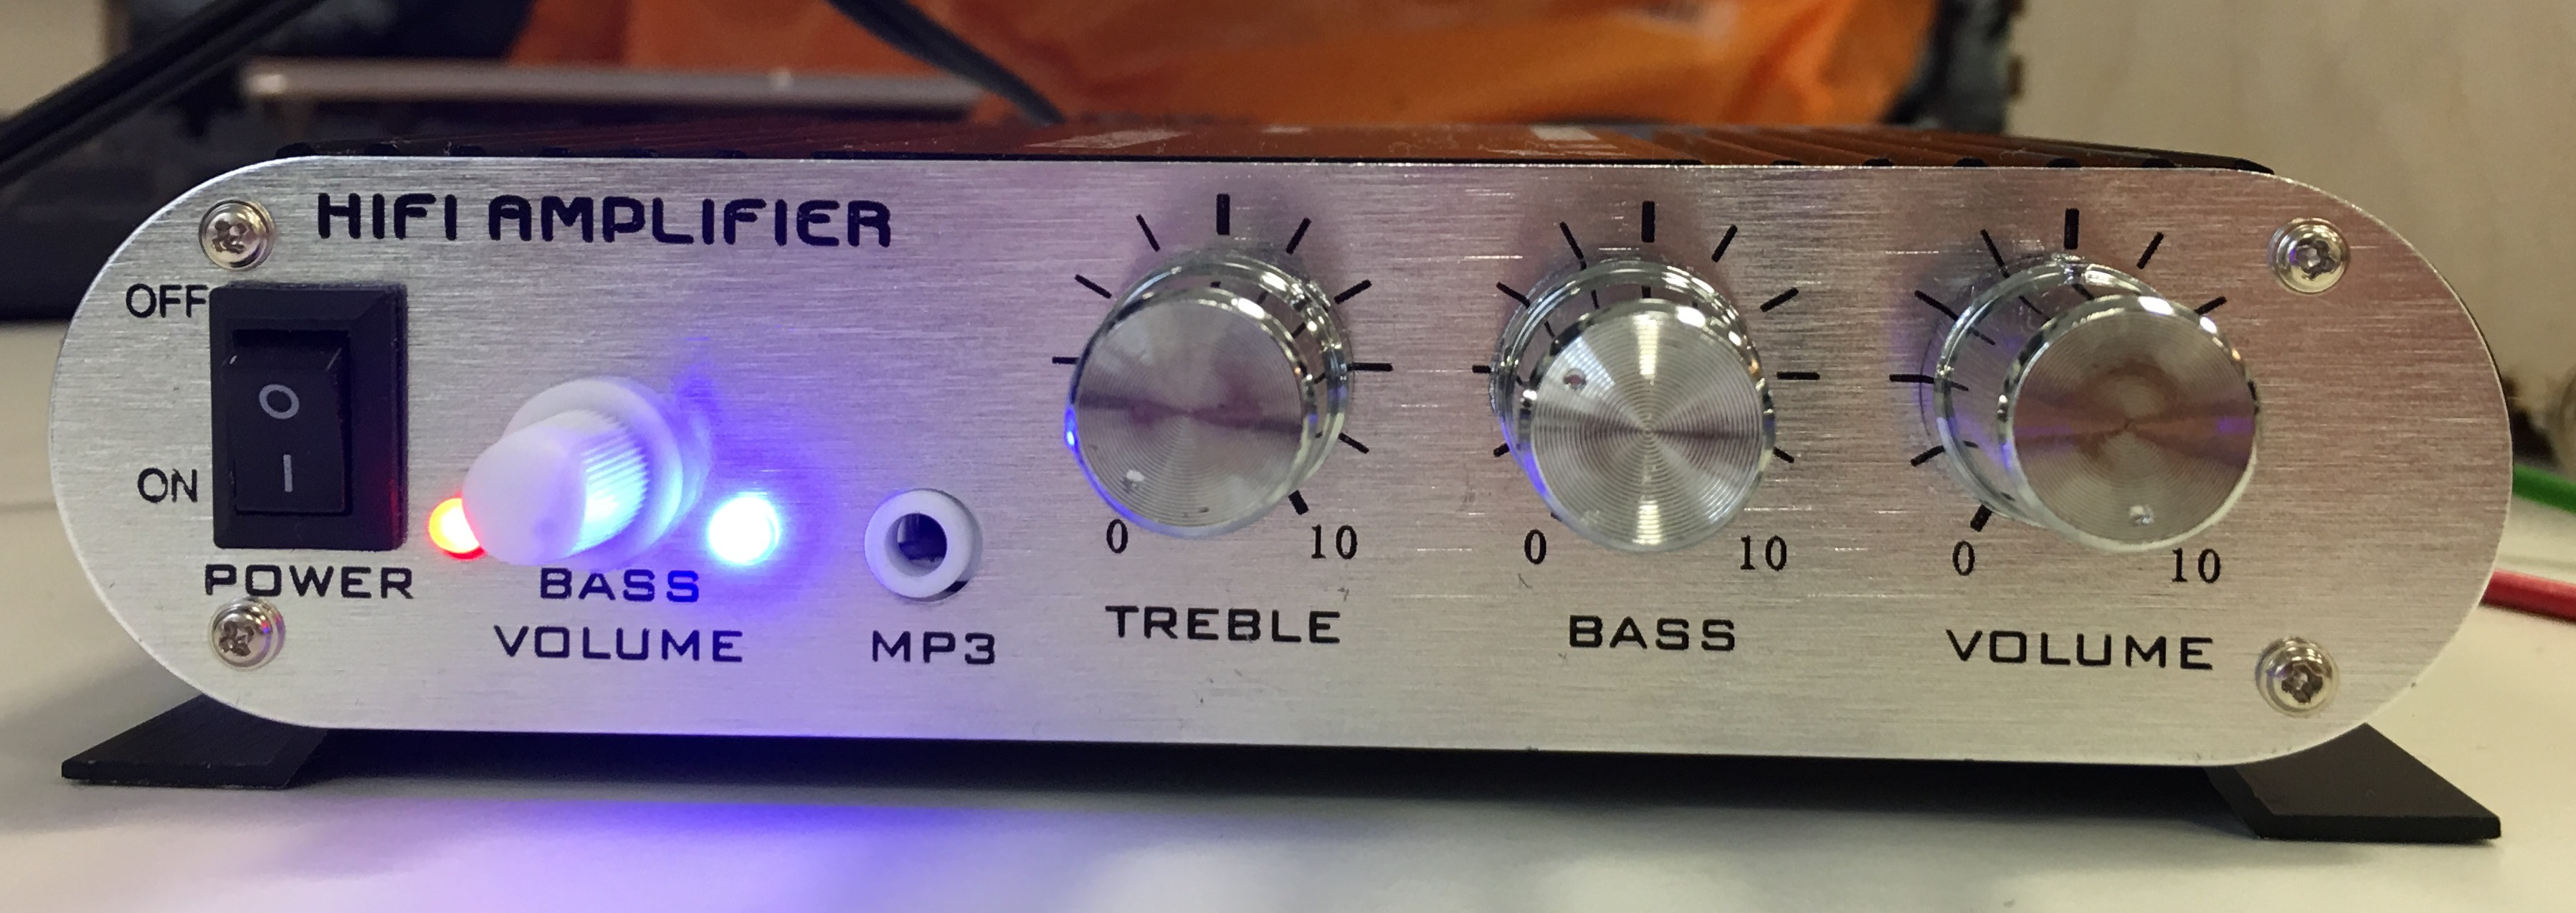
\includegraphics[width=\textwidth]{prototype/exp_rep_imgs/amp_controls.jpg}
        \caption{Image detailing the layout and variety of controls available to us with the amplifier.}
    \end{subfigure}
\caption{Images of the ELEGIANT Mini 20W 12V Hi-Fi Car Stereo Amplifier used to boost the input from the signal generator, in order to allow for vibrations of sufficient magnitude to produce droplet motion.}
\label{fig:amplifier}
\end{figure}

\begin{figure}[ht]
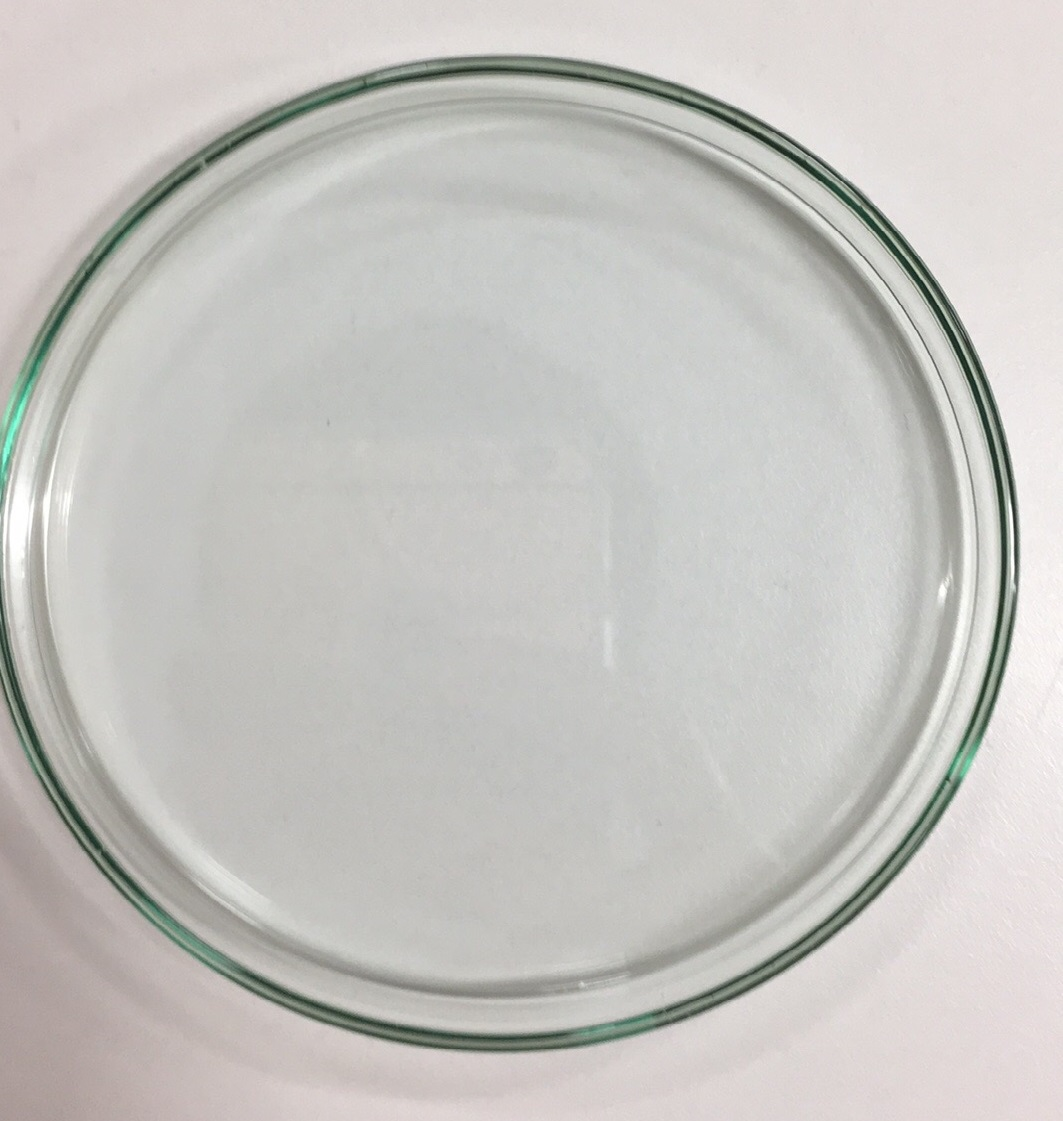
\includegraphics[width=12cm]{prototype/exp_rep_imgs/petriDish.jpg}
\centering
\caption{An image of the 4" petri dish used to house the liquid used as a surface in this experiment.}
\centering
\label{fig:PetriDish}
\end{figure}

\begin{figure}[ht]
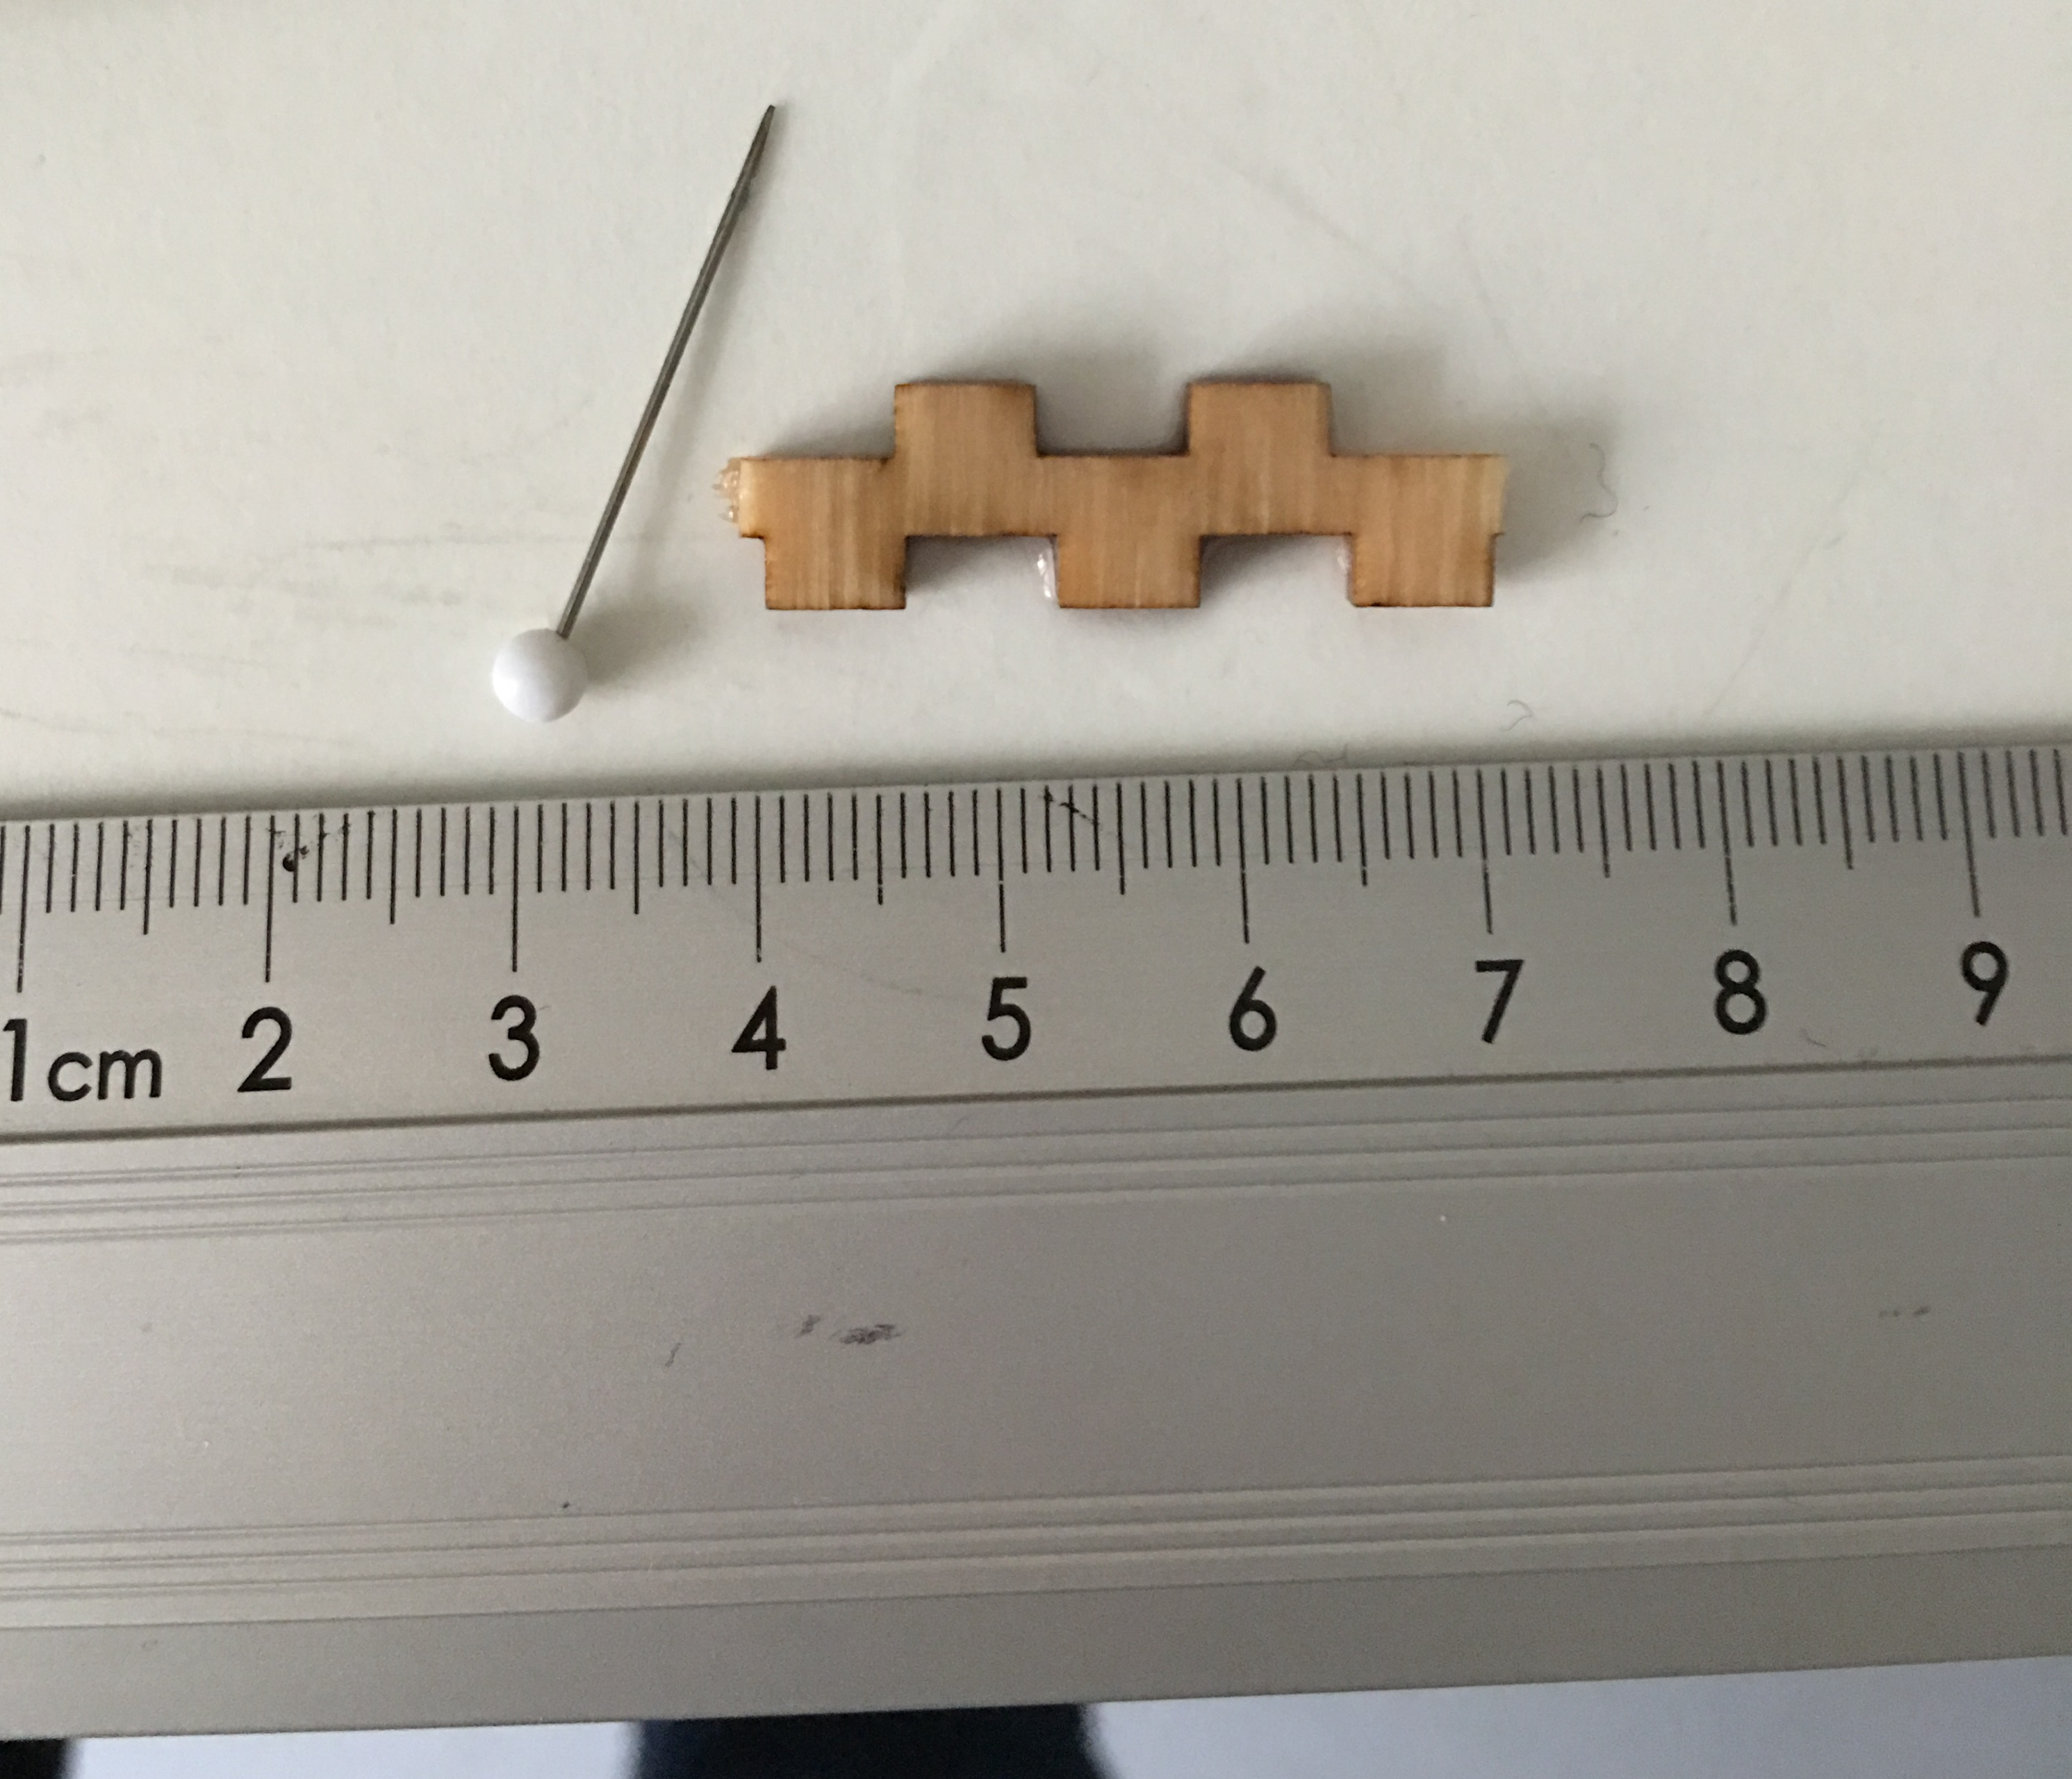
\includegraphics[width=12cm]{prototype/exp_rep_imgs/DropletCreators.jpg}
\centering
\caption{An image of a needle and glued together plywood remnant of the laser-cutting process, used to generate droplets for experimentation.  The plywood remnant was well suited to producing multiple droplets consistently, but using the needle to produce droplets proved to be difficult. It was instead utilised to destroy unwanted droplets. A ruler is placed alongside for scale  }
\centering
\label{fig:DropletCreators}
\end{figure}

\begin{figure}[ht]
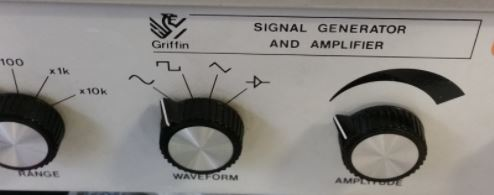
\includegraphics[width=12cm]{prototype/exp_rep_imgs/griffinsSigGen.jpg}
\centering
\caption{An image of the Griffins Signal generator initially used in this experiment. It had a in-built amplifier that helped boost the signal.}
\centering
\label{fig:griffinsSigGen}
\end{figure}

\begin{figure}[ht]
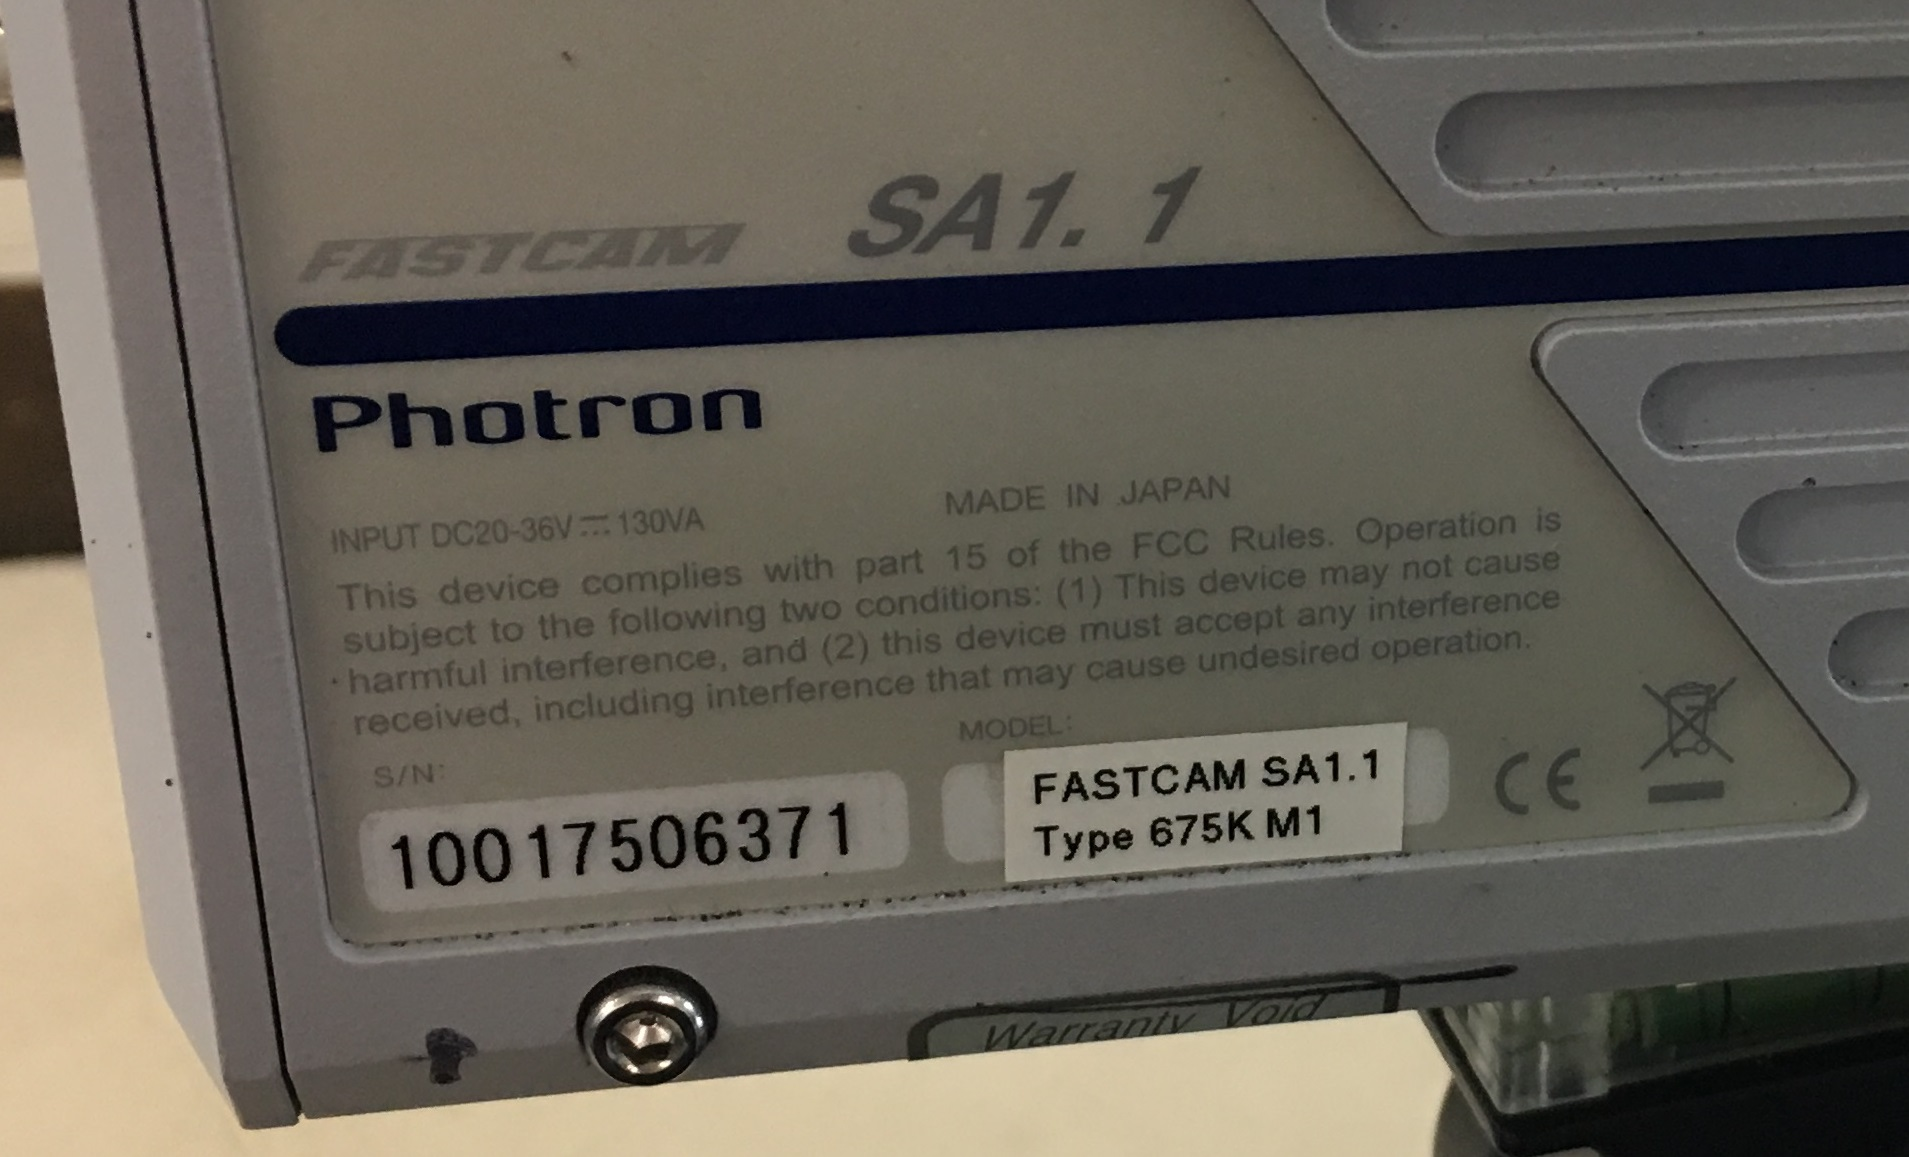
\includegraphics[width=12cm]{prototype/exp_rep_imgs/PhotronHighSpeedCamera.jpg}
\centering
\caption{Side view of the Photron Fastcam SA1.1 Type 675K M1 high speed camera used to capture the droplet motion at 1000 fps. The camera was controlled via a laptop installed with PFV Ver.3681, where settings such as resolution and frame rate could be modified.}
\centering
\label{fig:PhotronCamera}
\end{figure}

\begin{figure}[ht]
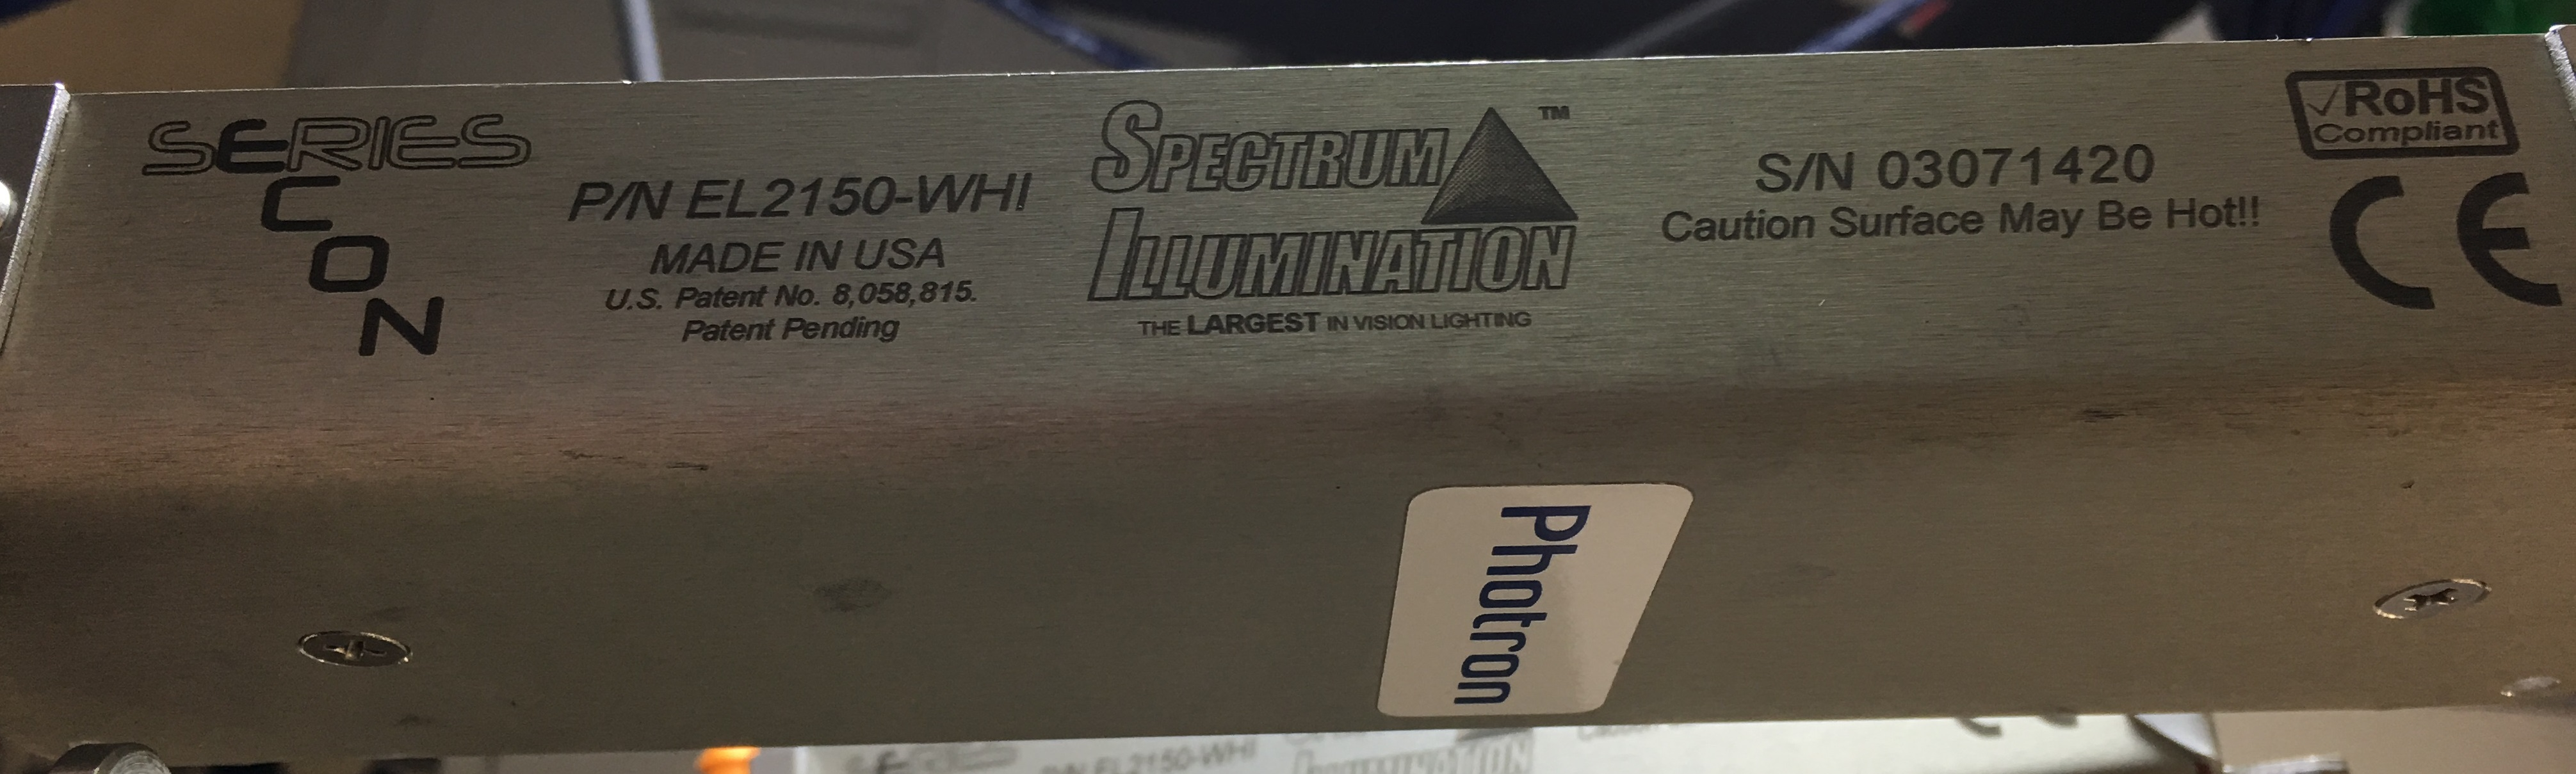
\includegraphics[width=12cm]{prototype/exp_rep_imgs/PhotronLighting.jpg}
\centering
\caption{Photron Spectrum Lumination P/N EL2150-WHI lighting uused to illuminate the droplets for high speed recording. The use of powerful lights is necessary to ensure clear recordings/images for high speed recording, due to the high shutter time and low light exposure.}
\centering
\label{fig:PhotronLighting}
\end{figure}

\subsection{Sourcing of Equipment}

To construct a preliminary experimental setup, the topic was investigated by an online search, and subsequent review of peer-reviewed papers. A list of equipment was compiled, with prices and links for purchase. This was partnered with alternative options as backups, in case of time concerns, budgeting issues or extensions to the experiment. Due to the limited budget of \pounds200, it was decided that the team would try to source as much of the equipment as possible for free. This was particularly vital, considering the preliminary fixed cost of \pounds40 that had to be set aside for poster printing.

The following steps were taken by our team in self-sourcing of equipment. This was to gain knowledge on certain equipment, borrowing them or seeking further assistance.

\begin{enumerate}
\item  Contact was made with the Mechanical Engineering department on the 5th floor of  Roberts building. We were able to order an `off the shelf' amplifier.  They were also able to provide us with a 3.5 mm jack to aux cable.
\item  Contact was made with Mychal Riley from Mechanical Engineering to enquire about borrowing a high speed camera. He provided us with a contact - Dr. Han Wu from 224  Chemical Engineering, who was in possession of a suitable device.
\item  After further exploration of the offices on the 4th floor of Roberts  building, a person referred us to Andrew Redfearn, who had equipment for professional video capturing.
\item  Contact was made with the owner of a camera shop near Tottenham Court Road station  - Parl Cameras: Rathbone Pl, Fitzrovia, London W1T 1JR
\item  A petri dish (4") was borrowed from the Chemistry department, from the Turner Lab  on the 2nd floor of Christopher Ingold building.
\end{enumerate}

The central piece of equipment was the loudspeaker. The main considerations were the power, dimensions and functions. It was decided that online purchases should be carried out with Amazon Prime due to its next day delivery service. The speaker was a 902.423UK 20W Woofer manufactured by QTX. The packaging and the actual device itself are displayed in Figure \ref{fig:speaker}.

Structural integrity and the ease of replicability were our primary considerations when designing the housing for the speaker and petri mount. After consulting staff at the Institute of Making (IoM), it was decided that laser cutting a template out of laser grade plywood would fulfil our base requirements. By using the free laser cutting case designer wasp provided by MakerCase (\url{http://www.makercase.com}), a template for the housing was generated. This allowed the housing to be replicable provided that access to a laser cutter and laser grade plywood was available. By incorporating finger joints in the design, the housing was sturdy enough to retain structural integrity when driving the speaker at maximum power output within the frequency range used without any adhesive or screws. The blueprint for the template is shown in Figure \ref{fig:blueprint}. It was designed to match laser grade plywood of 3 mm thickness.

\begin{figure}[htbp]
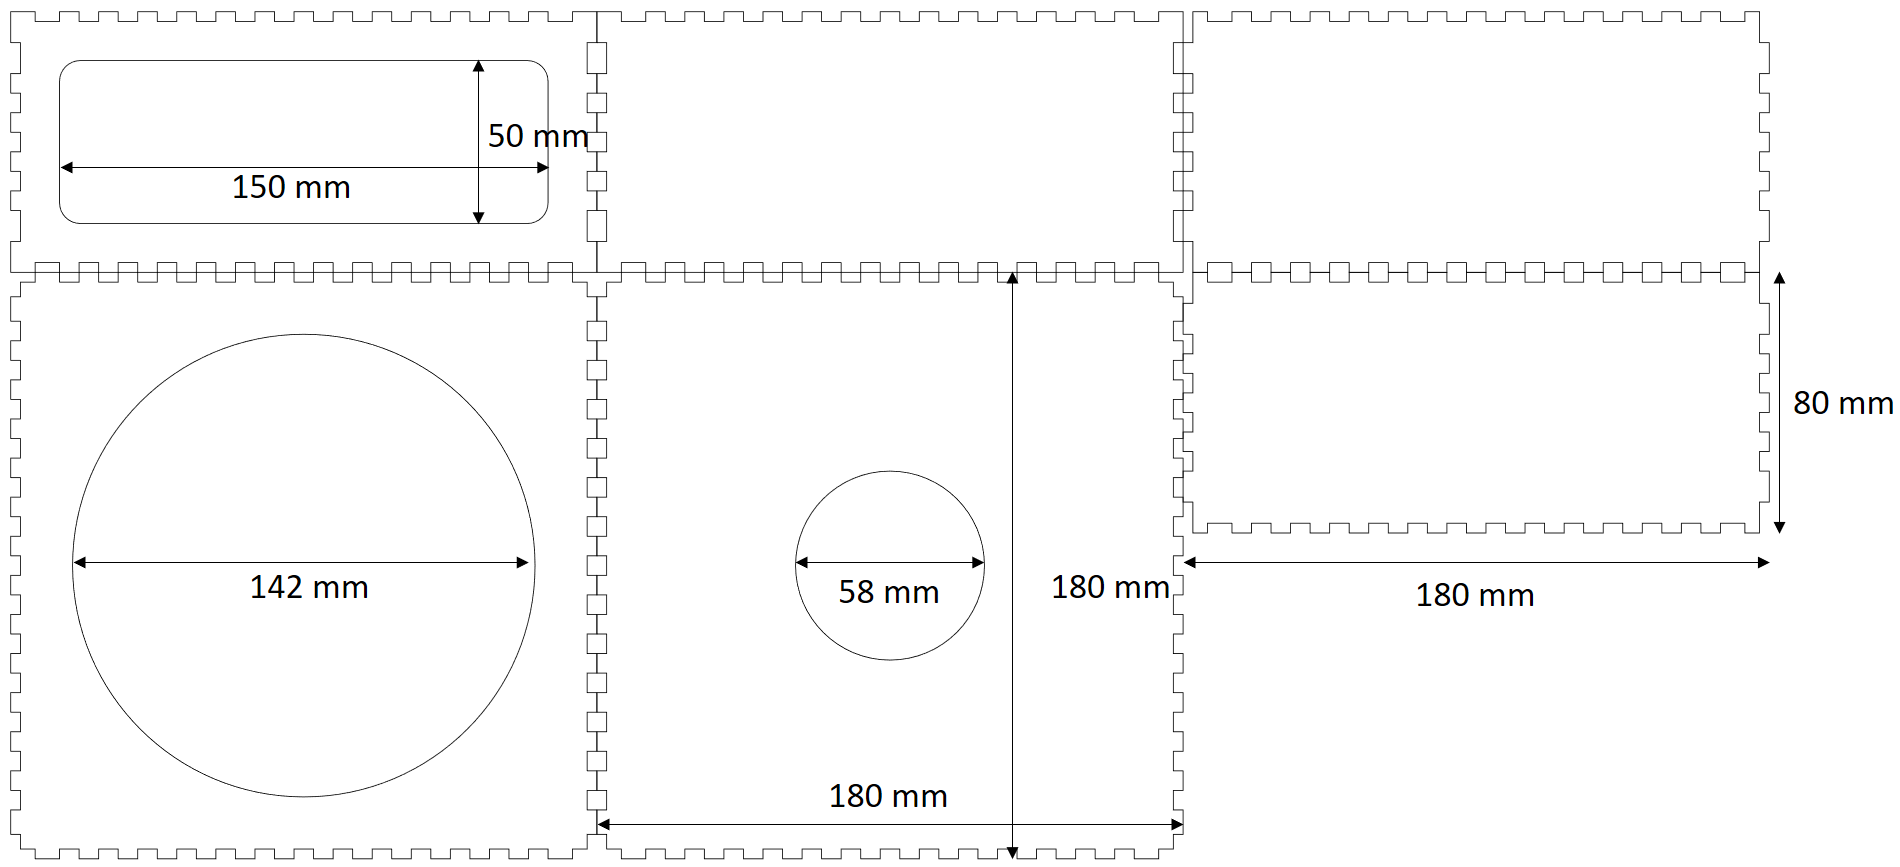
\includegraphics[width=\textwidth]{prototype/exp_rep_imgs/Blueprint.png}
\centering
\caption{Blueprint used in laser cutting the box that was used to house the loudspeaker. The blueprint provides the exact dimensions for the different components of the box before they were attached together.  }
\centering
\label{fig:blueprint}
\end{figure}

Measurement errors in the template resulted in the housing being 6mm too short for the speaker, causing the base of the speaker to protrude slightly out of the housing, thus making the housing unevenly balanced. To account for the height issue, two 3mm pieces of plywood were glued together and cut into 4 narrow strips. The strips were then glued to the housing to act as supporting platforms to hold up the speaker. To correct for the protruding speaker base, an additional copy of the bottom face of the housing was cut and glued onto the base of the housing. This ensured that the housing was properly levelled.

Were we afforded more time, we would ideally use a stronger material to  re-print the housing, possibly with stabilisers or a damping material, so that vibrations are driven directly into the fluid more efficiently rather than the box or surrounding platform. This perhaps could have been achieved by layering the base of the speaker with sand to damp unwanted vibrations.

The next step involves placing the speaker into the box. This process can be seen in Figure \ref{fig:boxassembly}.

\begin{figure}[ht]
\centering
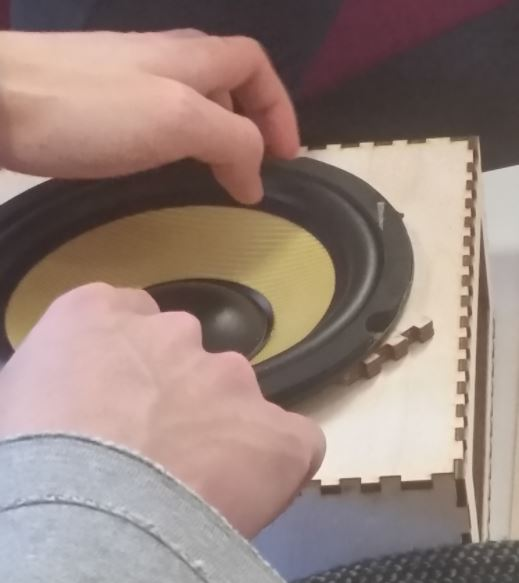
\includegraphics[width=0.5\textwidth]{prototype/exp_rep_imgs/boxAssembly.jpg}
\caption{A snapshot of the loudspeaker mounting process undertaken as part of the initial assembly stage. One of the cut pieces of plywood used to support the speaker is also visible here.}
\label{fig:boxassembly}
\end{figure}


\subsection{Testing of Loudspeaker}
Preliminary testing was conducted using an ISO-TECH synchronized function generator GFG2004. A detectable signal was picked up by the loudspeaker, where the diaphragm was clearly vibrating and producing sound. However, the signal was found to be too weak to cause vibrations in a petri dish. The team then tried to source a function generator that offered a higher output power. The Physics Laboratory was able to provide a Griffin function generator that allowed for amplification. It was decided that the team would have to attempt produce droplets with this function generator before purchasing an amplifier.

\subsection{Experimentation with 1000 cSt silicone oil}
A full experimental run  was carried out by connecting the Griffin function generator to the loudspeaker, in order to drive a petri dish of 1000 cSt silicone oil. Double sided tape was used to stick a square cardboard plate onto the loudspeaker's edge/diaphragm intersection and then sticking the petri dish onto the cardboard. This was to avoid damaging the diaphragm. However a concern was raised regarding the ability of the cardboard plate to fully transmit the vibration of the loudspeaker. Sticking the petri dish onto the diaphragm with adhesive was considered as a final resort.

About 4 mm of silicone oil was poured into the 4'' petri dish. This was measured using a metal ruler that was aligned to the base of the petri dish. A frequency range of 50 -- 100 Hz was tested, adjusted via the frequency generator.

Using a needle to quickly flick the surface of the oil, unsuccessful attempts were made to produce droplets. This was thought to be due to the high viscosity of the oil, as droplets were observed to stay on the tip of the needle even after rigorous attempts to dislodge them. In the rare occasions where droplets were actually produced, they did not last for long before coalescing with the liquid. The droplet diameter was also very large ($>$1mm) and the droplets appeared to be sitting on the surface instead of bouncing. Different methods were tried, including releasing droplets from a low height. However there was little chance to observe actual bouncing, or to produce sustainable droplets in order to test other phenomena.

As a result,  many possible improvements were considered. It was not clear what the major problem was, but it  could have been caused by the low driving amplitude, which did not provide enough acceleration to allow for bouncing. The other was the high viscosity of silicone oil. It was also decided that the square cardboard plate had to be replaced due to its lack of rigidity. Air was observed to escape from the side of the loudspeaker, which meant that energy was lost and not transmitted to the petri dish. 

It was decided that improvements were to be carried out immediately, hence the decision to purchase an ELEGIANT qroiip2097 20W amplifier. This was accompanied by a Sunydeal 60W power cable.

The cardboard plate was replaced with a circular 3 mm thick plywood cut-out, a by-product of the laser-cutting process. It was found that the diameter was slightly too small, as it was not able to reach the outer edge of the loudspeaker. Despite this, the new plywood plate was still large enough to be secured with double-sided tape. 

A lower viscosity silicone oil (50 cSt) was obtained from the Turner Lab in the Chemistry Department. These improvements were subsequently incorporated into the equipment.

\subsection{Experimentation with 50 cSt silicone oil}
With the lower viscosity silicone oil and the improved setup, a second attempt was made to produce droplets. The amplifier knobs allowed the adjustment of treble, bass and volume. The amplifier input was connected to the function generator's output via a 3.5 mm jack to aux cable and a pair of banana plugs. The output was connected to the loudspeaker's input with banana plugs. This setup can be seen in Figure \ref{fig:exp_setup_sideshot}.

\begin{figure}[ht]
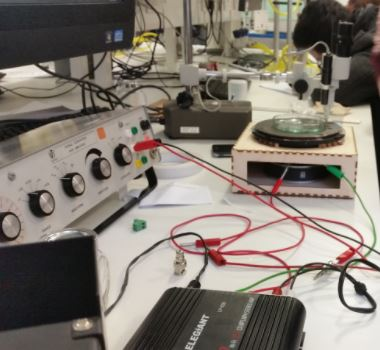
\includegraphics[width=0.5\textwidth]{prototype/exp_rep_imgs/exp_setup_sideshot.jpg}
\centering
\caption{The experimental setup in testing the 50 cSt silicone oil. This setup used an amplifier connected to the Griffin function generator, and the amplifier output was connected to the loudspeaker via crocodile clips.  }
\centering
\label{fig:exp_setup_sideshot}
\end{figure}

To maximise the transmitted signal, the function generator was set to minimum attenuation and connected via the 4 ohms impedance output to match the impedance of the speaker. A smart phone was also tested. The results were very similar to that of the function generator, but the phone provides an advantage in terms of accessibility and ease of use.

The output wave was tested in a frequency range of 50 -- 80 Hz. Bouncing droplets that persisted for minutes were produced. High volume and bass were found to be beneficial for producing high-bouncing droplets. It was discovered that the frequency range corresponded to bass, thus both knobs work similarly.

Some droplets also appeared to 'walk'. However it was uncertain if they were indeed exhibiting a 'walking' phenomenon or was it due to an external force. This is because any form of breeze in the laboratory could easily move the droplets; talking could also have produced enough pressure to move them. It was also possible to combine droplets together, forming crystal lattice-like structures.

Using the slow-motion video capturing mode on iPhone, the droplet behaviour and motion were captured. It was found that the droplet size was too small to be accurately determined by the naked eye or with a photograph. An alternate method was proposed: viewing the droplet through a microscope borrowed from Physics Lab 3. However after several attempts to focus the lens and lighting, it was found to be non-feasible, and the idea was not investigated further.

Improvements were proposed to improve the setup. It was decided that graph paper could be taped underneath the petri dish. The grid would provide a useful way to track the droplet's motion and size. Through the use of software, it would be possible to track the amplitude and thus develop a method to obtain quantitative results. The other concern was regarding the plywood base, which was only taped down, and thus is insecure. There were multiple times where it had to be held down by  hand as the vibrations were strong enough to tear the plate off the taped area. This suggested that objects that mimic clamps could be used to secure the plywood plate. A possible candidate was foldback clips and so Q-connect 42 mm  foldback clips were purchased.


These clips are common office stationary, and offer a very strong clamping ability. The primary advantage of these clips was their size. The clips had to be large enough to clamp a reasonable width, whilst not being large enough to come into contact with the petri dish. The plywood plate was also re-cut to fit the correct size of the loudspeaker edge, which would make it much easier for the clips to clamp on strongly.

\subsection{Dark Room Recording}
A lot of findings in this investigation were obtained using video footage. Bouncing and walking phenomena are very qualitative observations that are hard to quantify, so the best way to demonstrate them was through frame by frame representation. A mobile phone camera would not be able to perform up to this level, which is why a professional camera had to be sourced at this stage.

Contact was made with Andrew Redfearn, a Ph.D Engineering student who kindly agreed to let us use his digital camera (Sony Cyber-shot RX-100 IV) and the high powered lighting (TriLite Max 3x30W Compact Flourescent Lamps 220-240V) in his laboratory (Roberts UB54) to record some footage. The experiment was conducted in a dark room. Andrew's setup also included a trigger prompting 2 seconds of recording, which was relayed to a computer monitor, as shown in Figure \ref{fig:slowmo_setup}.

\begin{figure}[ht]
\centering
    \begin{subfigure}[t]{0.475\textwidth}
    \centering
        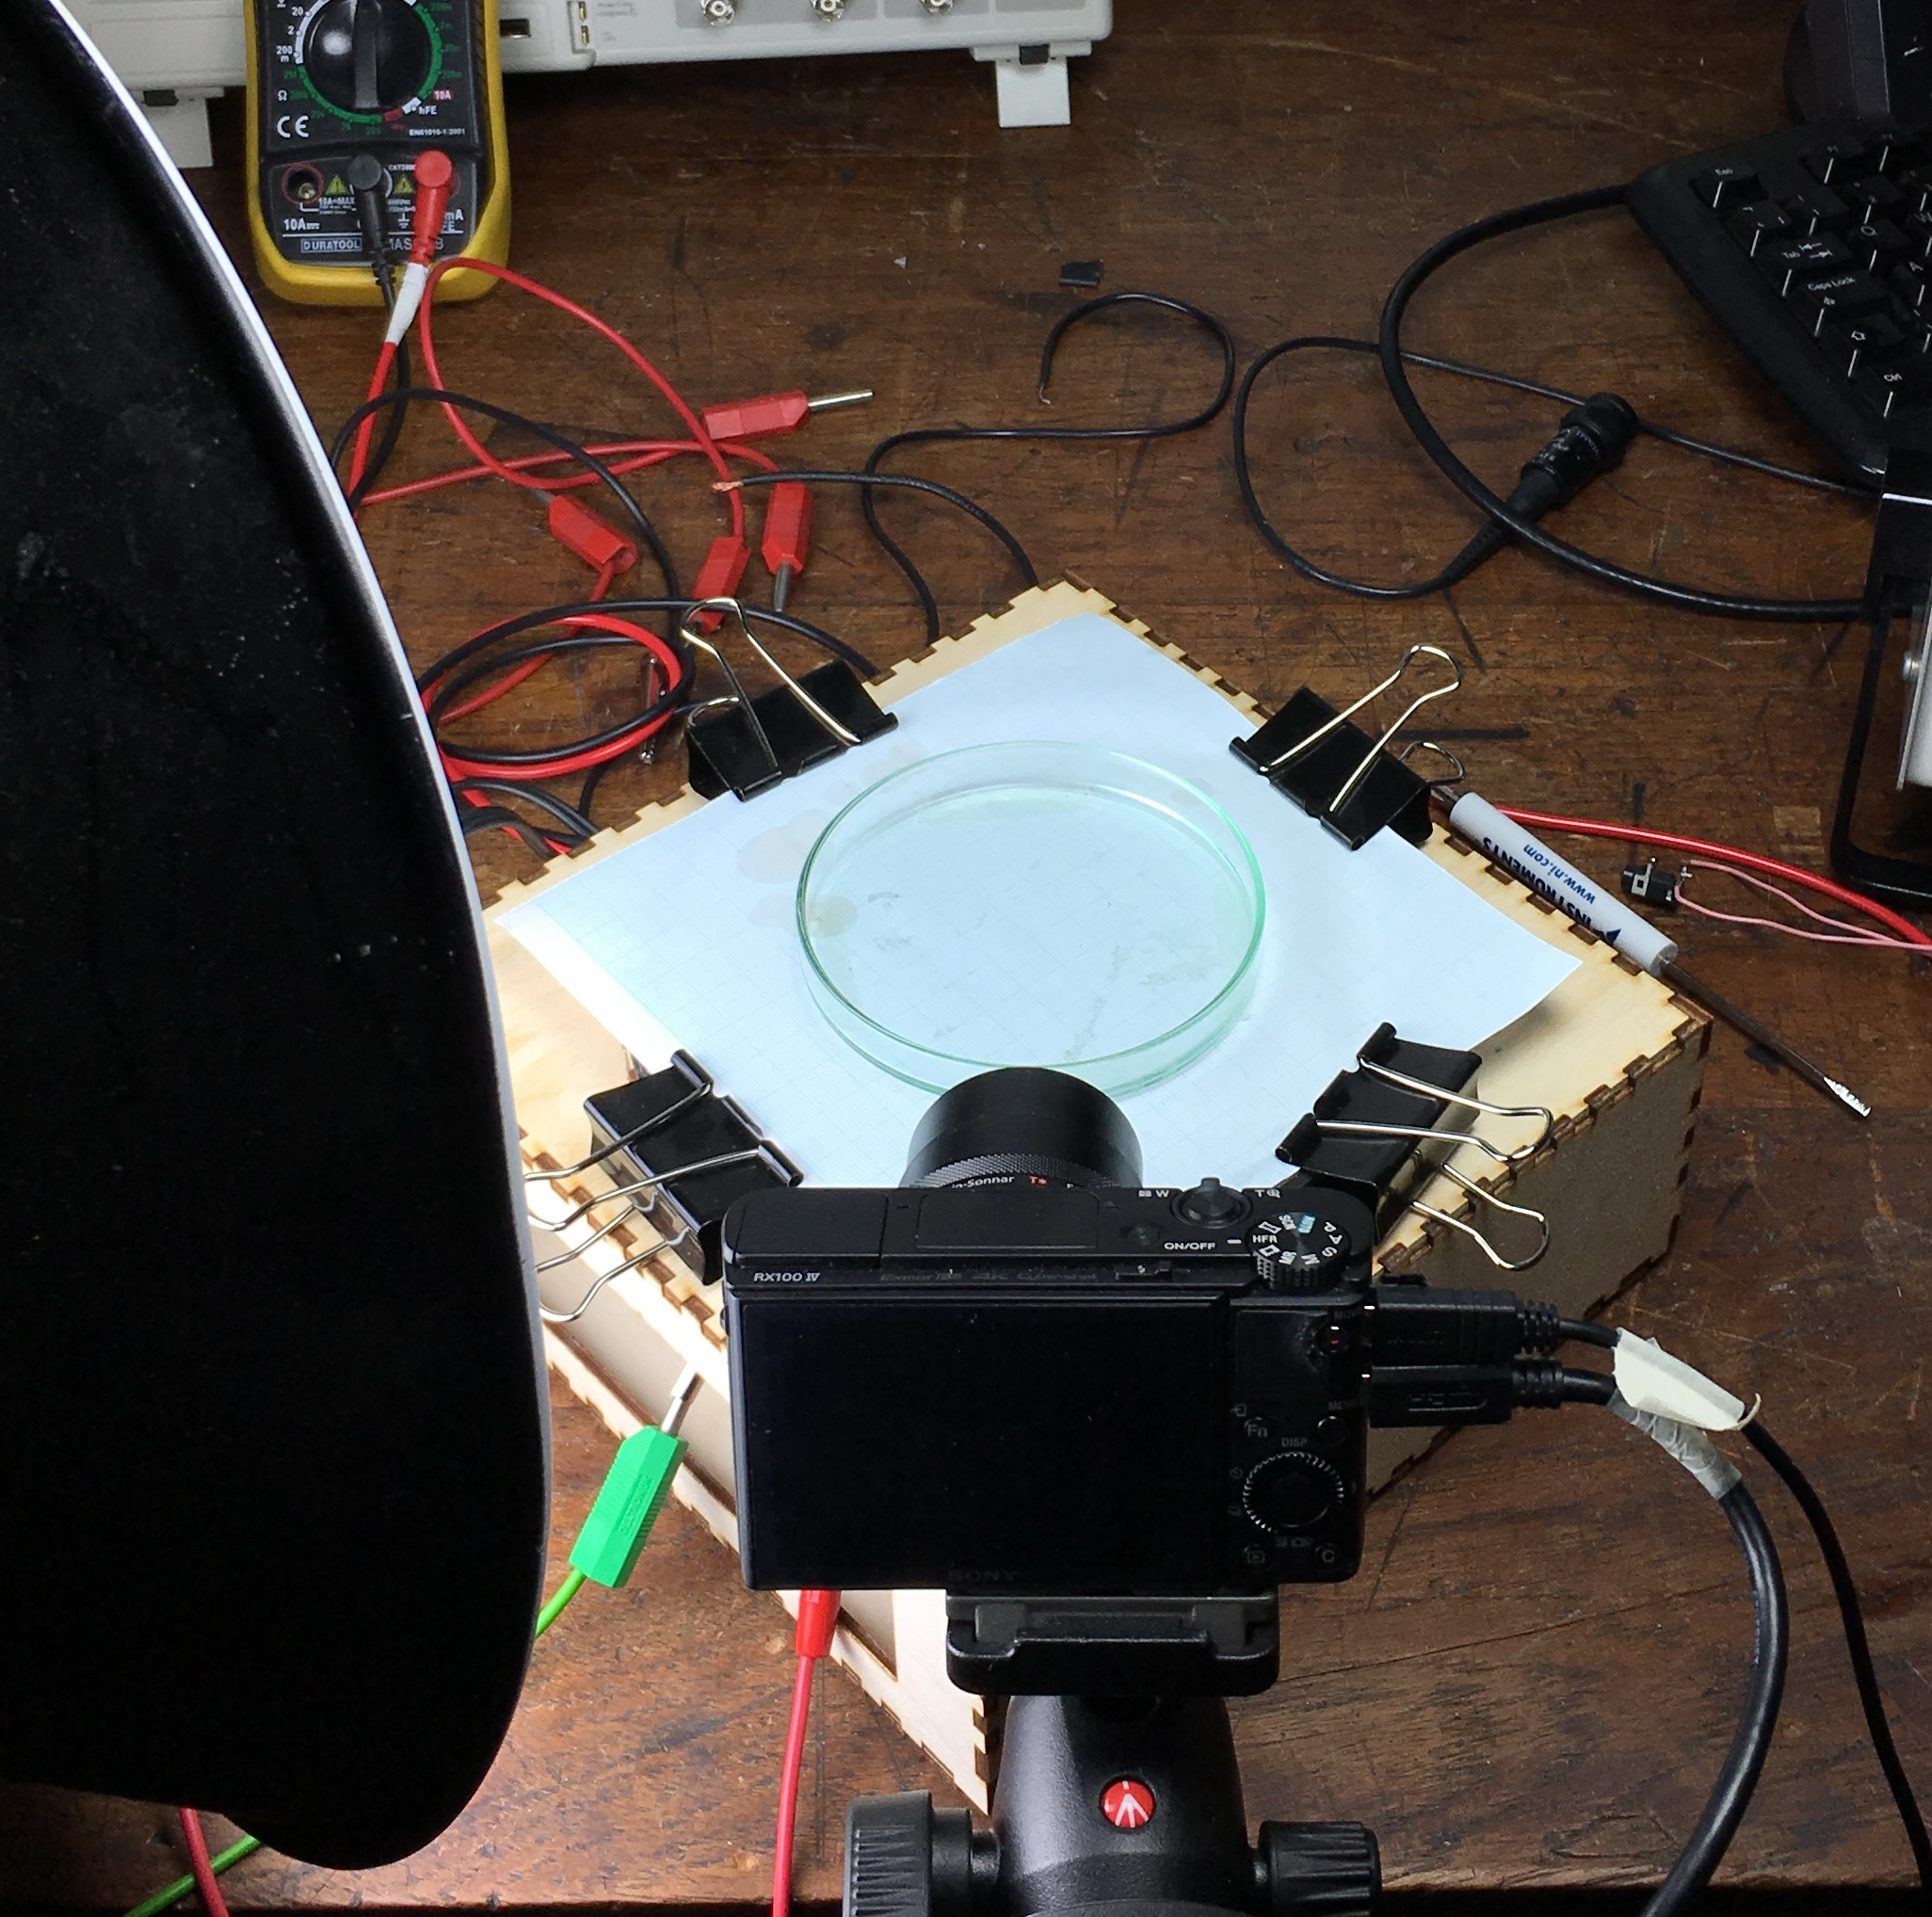
\includegraphics[width=\textwidth]{prototype/exp_rep_imgs/closeup_slowmo_setup.jpg}
        \caption{A closeup of the positioning of the camera and spotlight.}
    \end{subfigure}
    \begin{subfigure}[t]{0.475\textwidth}
    \centering
        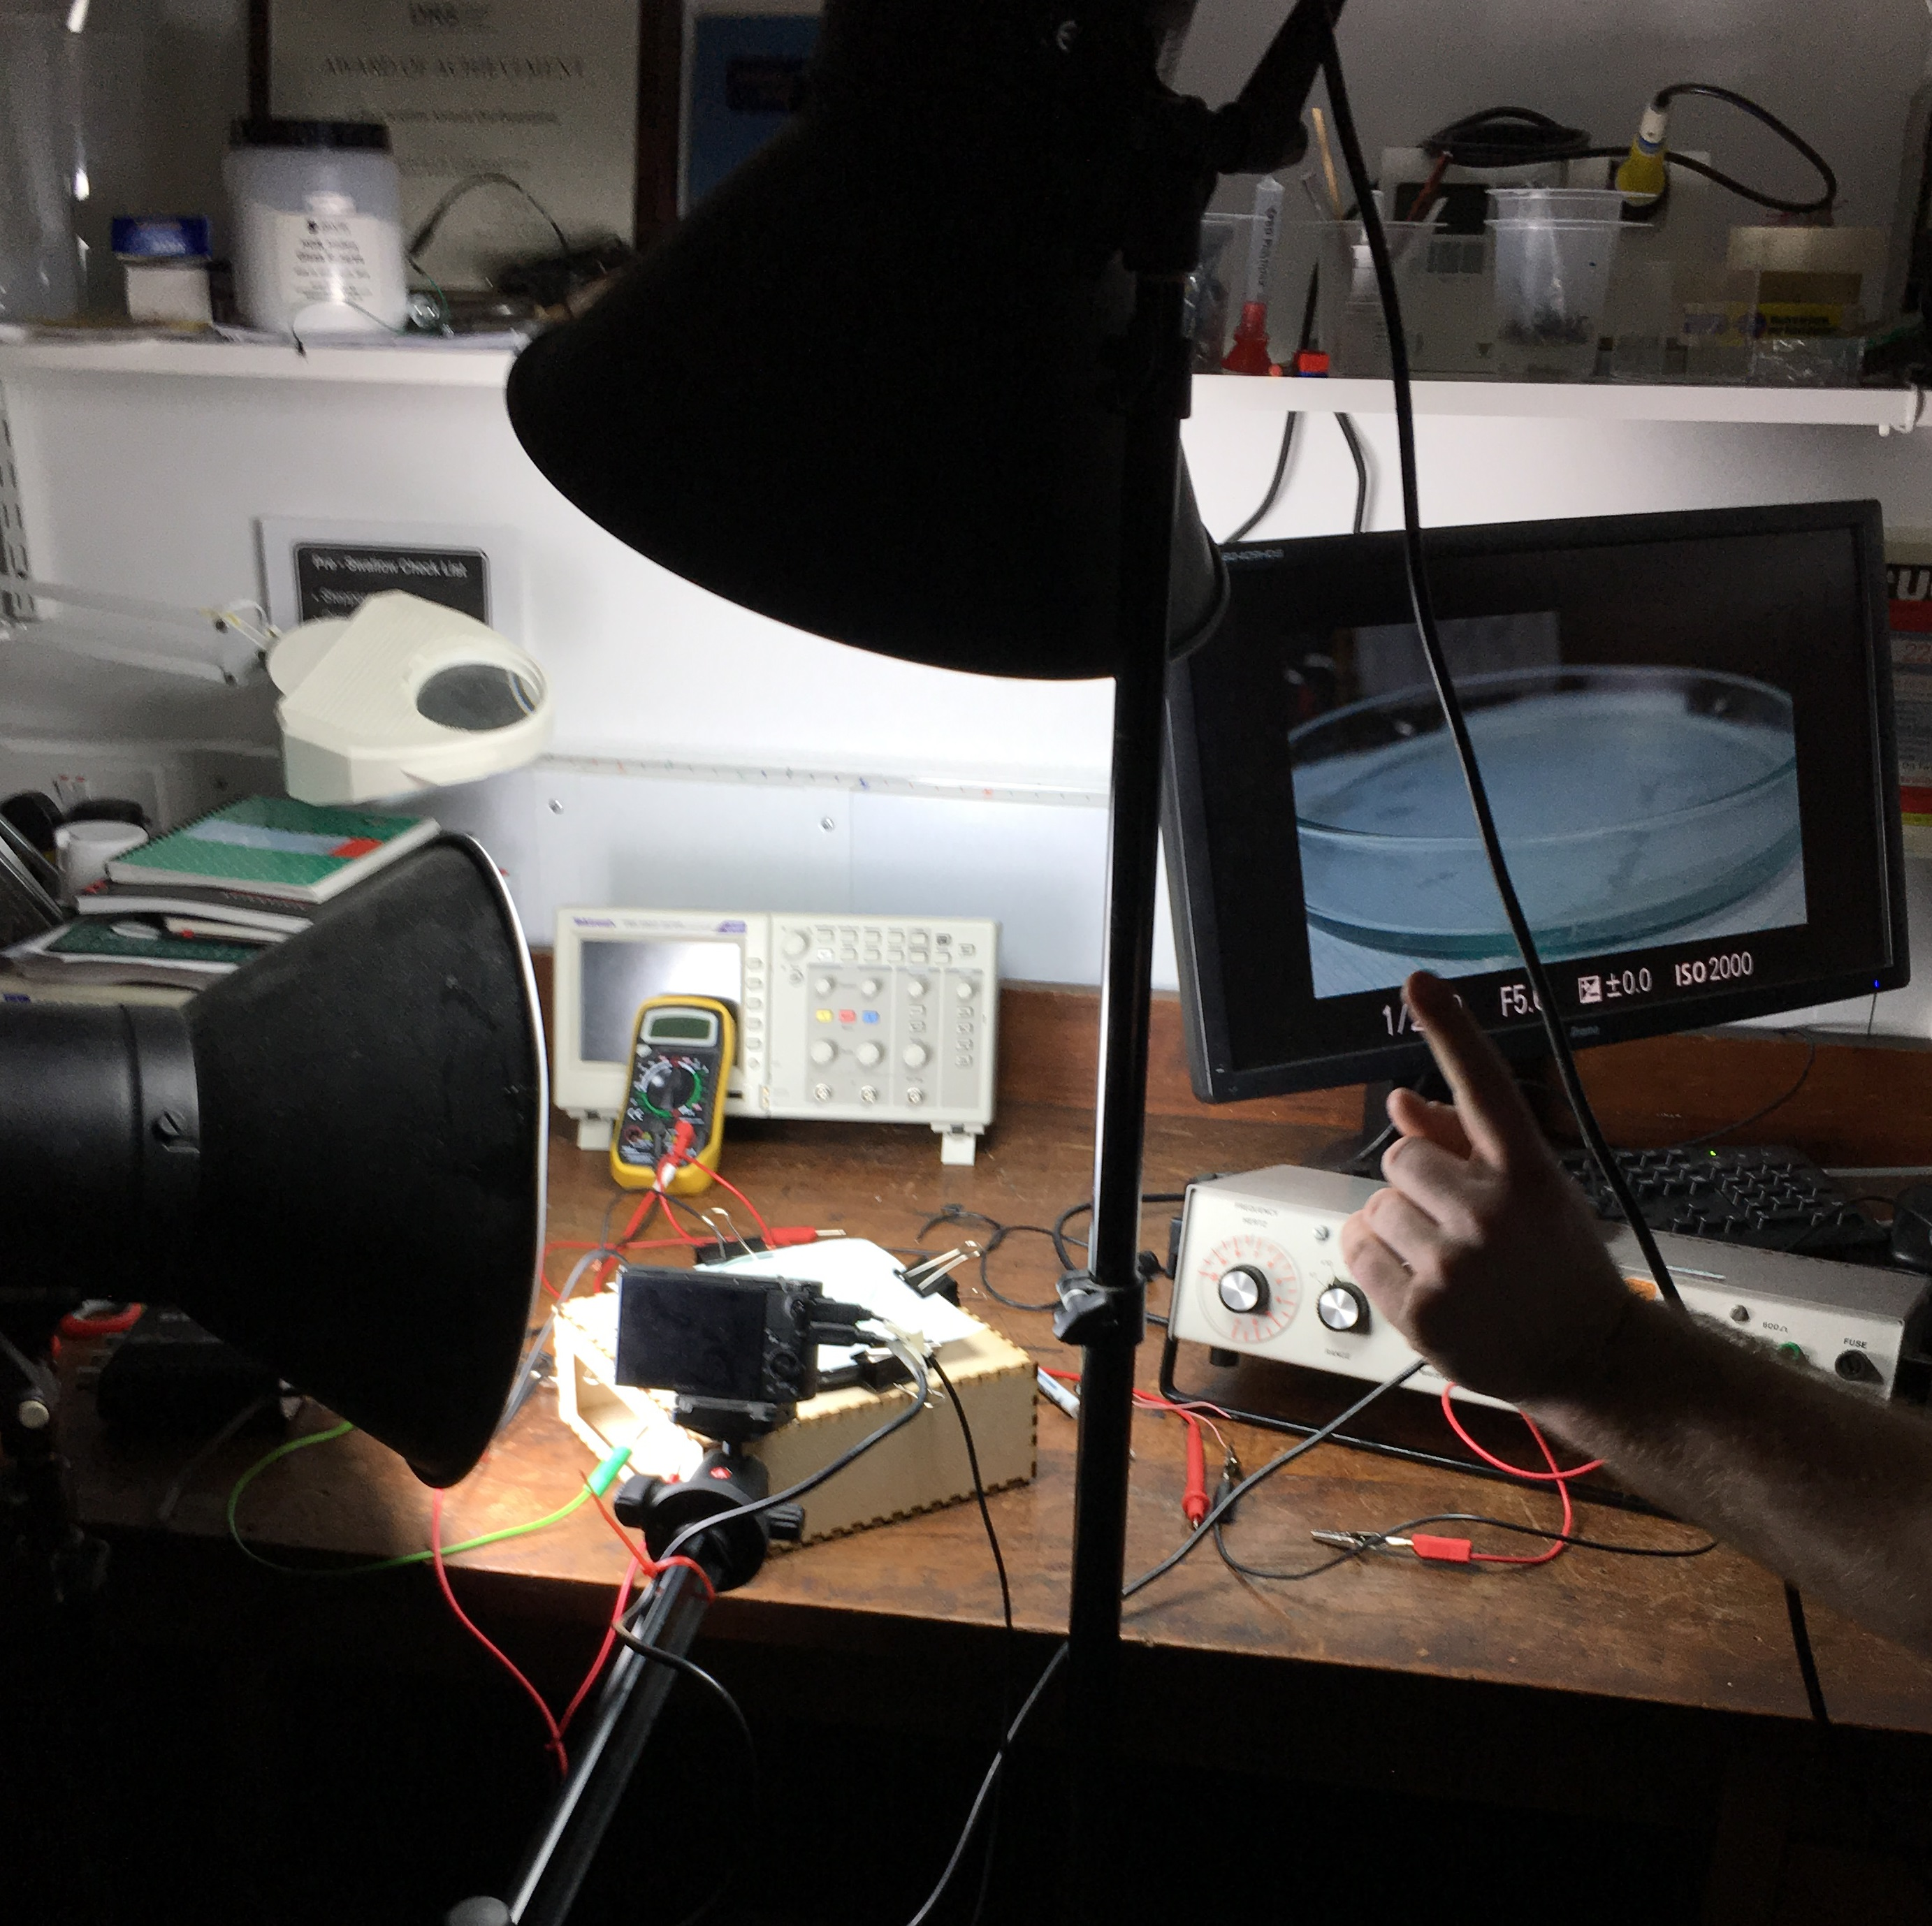
\includegraphics[width=\textwidth]{prototype/exp_rep_imgs/slowmo_setup.jpg}
        \caption{Full setup including the trigger and live recording on the computer monitor.}
    \end{subfigure}
\caption{The Sony Cyber-shot RX-100 IV Camera set up on a tripod, accompanied by spotlights for slow motion recording. }
\label{fig:slowmo_setup}
\end{figure}

Though the focusing was difficult at the start, it was resolved by forcing the droplets closer to the edge of the petri dish. Graph paper was taped underneath the petri dish to get an idea of the typical size of droplets. They were found to be approximately 1 mm in diameter. Recording was achieved at regular (25 fps) and high (50 fps) speeds through a frequency range of 50 -- 80 Hz. It was found that droplets were most stable at 50 Hz, which became the standard frequency used. As the strong lighting caused unwanted reflections, it was suggested that a polaroid or a diffuser be used to filter the light. This is analogous to wearing polarising sunglasses and being able to see fish in water more easily.

Interestingly, the bouncing itself was refracted through the glass and waves were observed on the bottom of the petri dish. This can be seen in Figure \ref{fig:bouncing_refr_glass}. Following this, research was carried out into the potential of motion tracking in obtaining quantitative data. It was found that Adobe AfterEffects offered this function. The method is summarised in the following steps:

\begin{enumerate}
\item  Creating a new null object to store the droplet coordinates
\item  Using the Track Camera, locate the region to track and then analyze  the clip.
\item  Apply the results to the null object.
\item  Select all key frames and paste in notepad.
\item  Plot in Excel.
\end{enumerate}

\begin{figure}[ht]
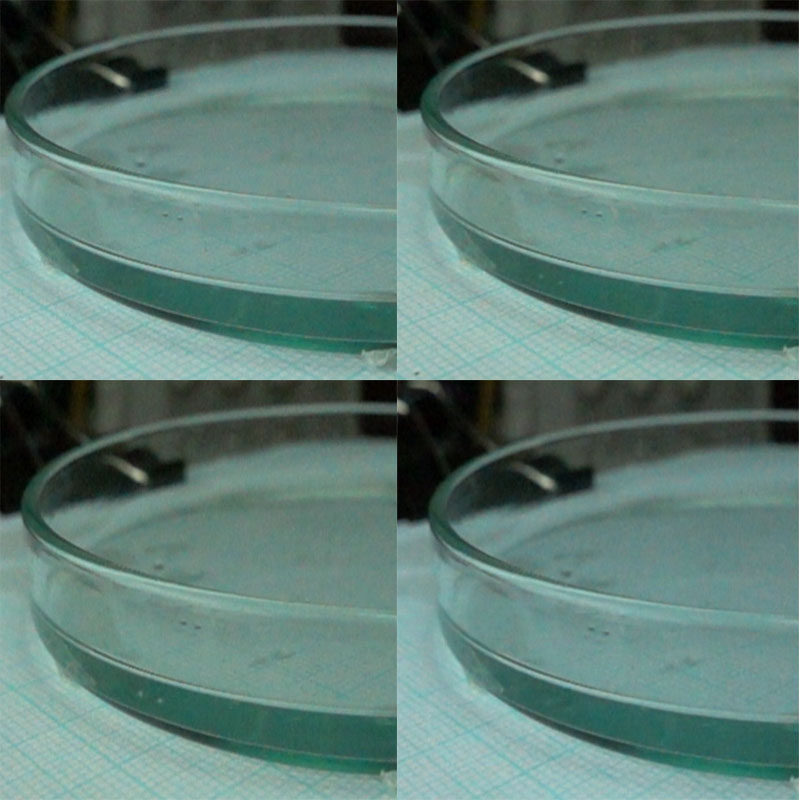
\includegraphics[width=\textwidth]{prototype/exp_rep_imgs/bouncing_refr_glass.jpg}
\centering
\caption{Four images displaying the bouncing motion refracted through the glass, captured using the Sony Cyber-shot RX-100 IV setup and 50 cSt silicone oil. With silicone oil, the droplets are hard to see, even with slow motion recording, due to their small size and transparent nature.}
\centering
\label{fig:bouncing_refr_glass}
\end{figure}

\subsection{Uncontrolled Experimental Factors}
During experimentation, attempts were made to observe walking and repelling pairs, in order to gain an idea of the typical amplifier volume needed to produce such phenomena. At the beginning, the temperature of the lab was measured. Low temperature led to a higher viscosity, which could have had an effect on droplet motion. Oil depth was also considered to be a factor.

Under normal lighting, the shadow of the droplet was projected on the graph paper when illuminated from above. This was used to obtain an estimate of the size of the droplet, although this was subject to parallax error as it had to be observed at an angle.

An attempt to determine the signal amplitude that created Faraday instability was made. A series of measurements of noise level were made at different distances for a fixed volume. This was to determine the sound level variation as a function of distance. The results were inconclusive, but it was decided that a fixed distance of 30 cm was to be used. Having a quantitative measure of noise level provided an alternative to measuring the acceleration. However, there was very little success in measuring the variation and a fixed noise level to achieve Faraday instability.

It was eventually decided that, due to the difficulty in trying to quantify measurements, it would be most effective to observe and record phenomena. This was deemed a path of greater success given the time frame for this project.

\subsection{Double slit diffraction}
Following these investigations, a resized plywood base was produced and fitted onto the loudspeaker with foldback clips. The use of tape was also eliminated as the clips were secure enough. Double slit diffraction was attempted by constructing a grating with rectangular wooden sticks. The petri dish was replaced with a square Tupperware box as shown in Figure \ref{fig:double_slit_setup} as it had a larger area and more flexibility with positioning the gratings. The width of slits was approximately equal to the size of the droplets.

\begin{figure}[h]
    \centering
    \begin{subfigure}{0.475\textwidth}
        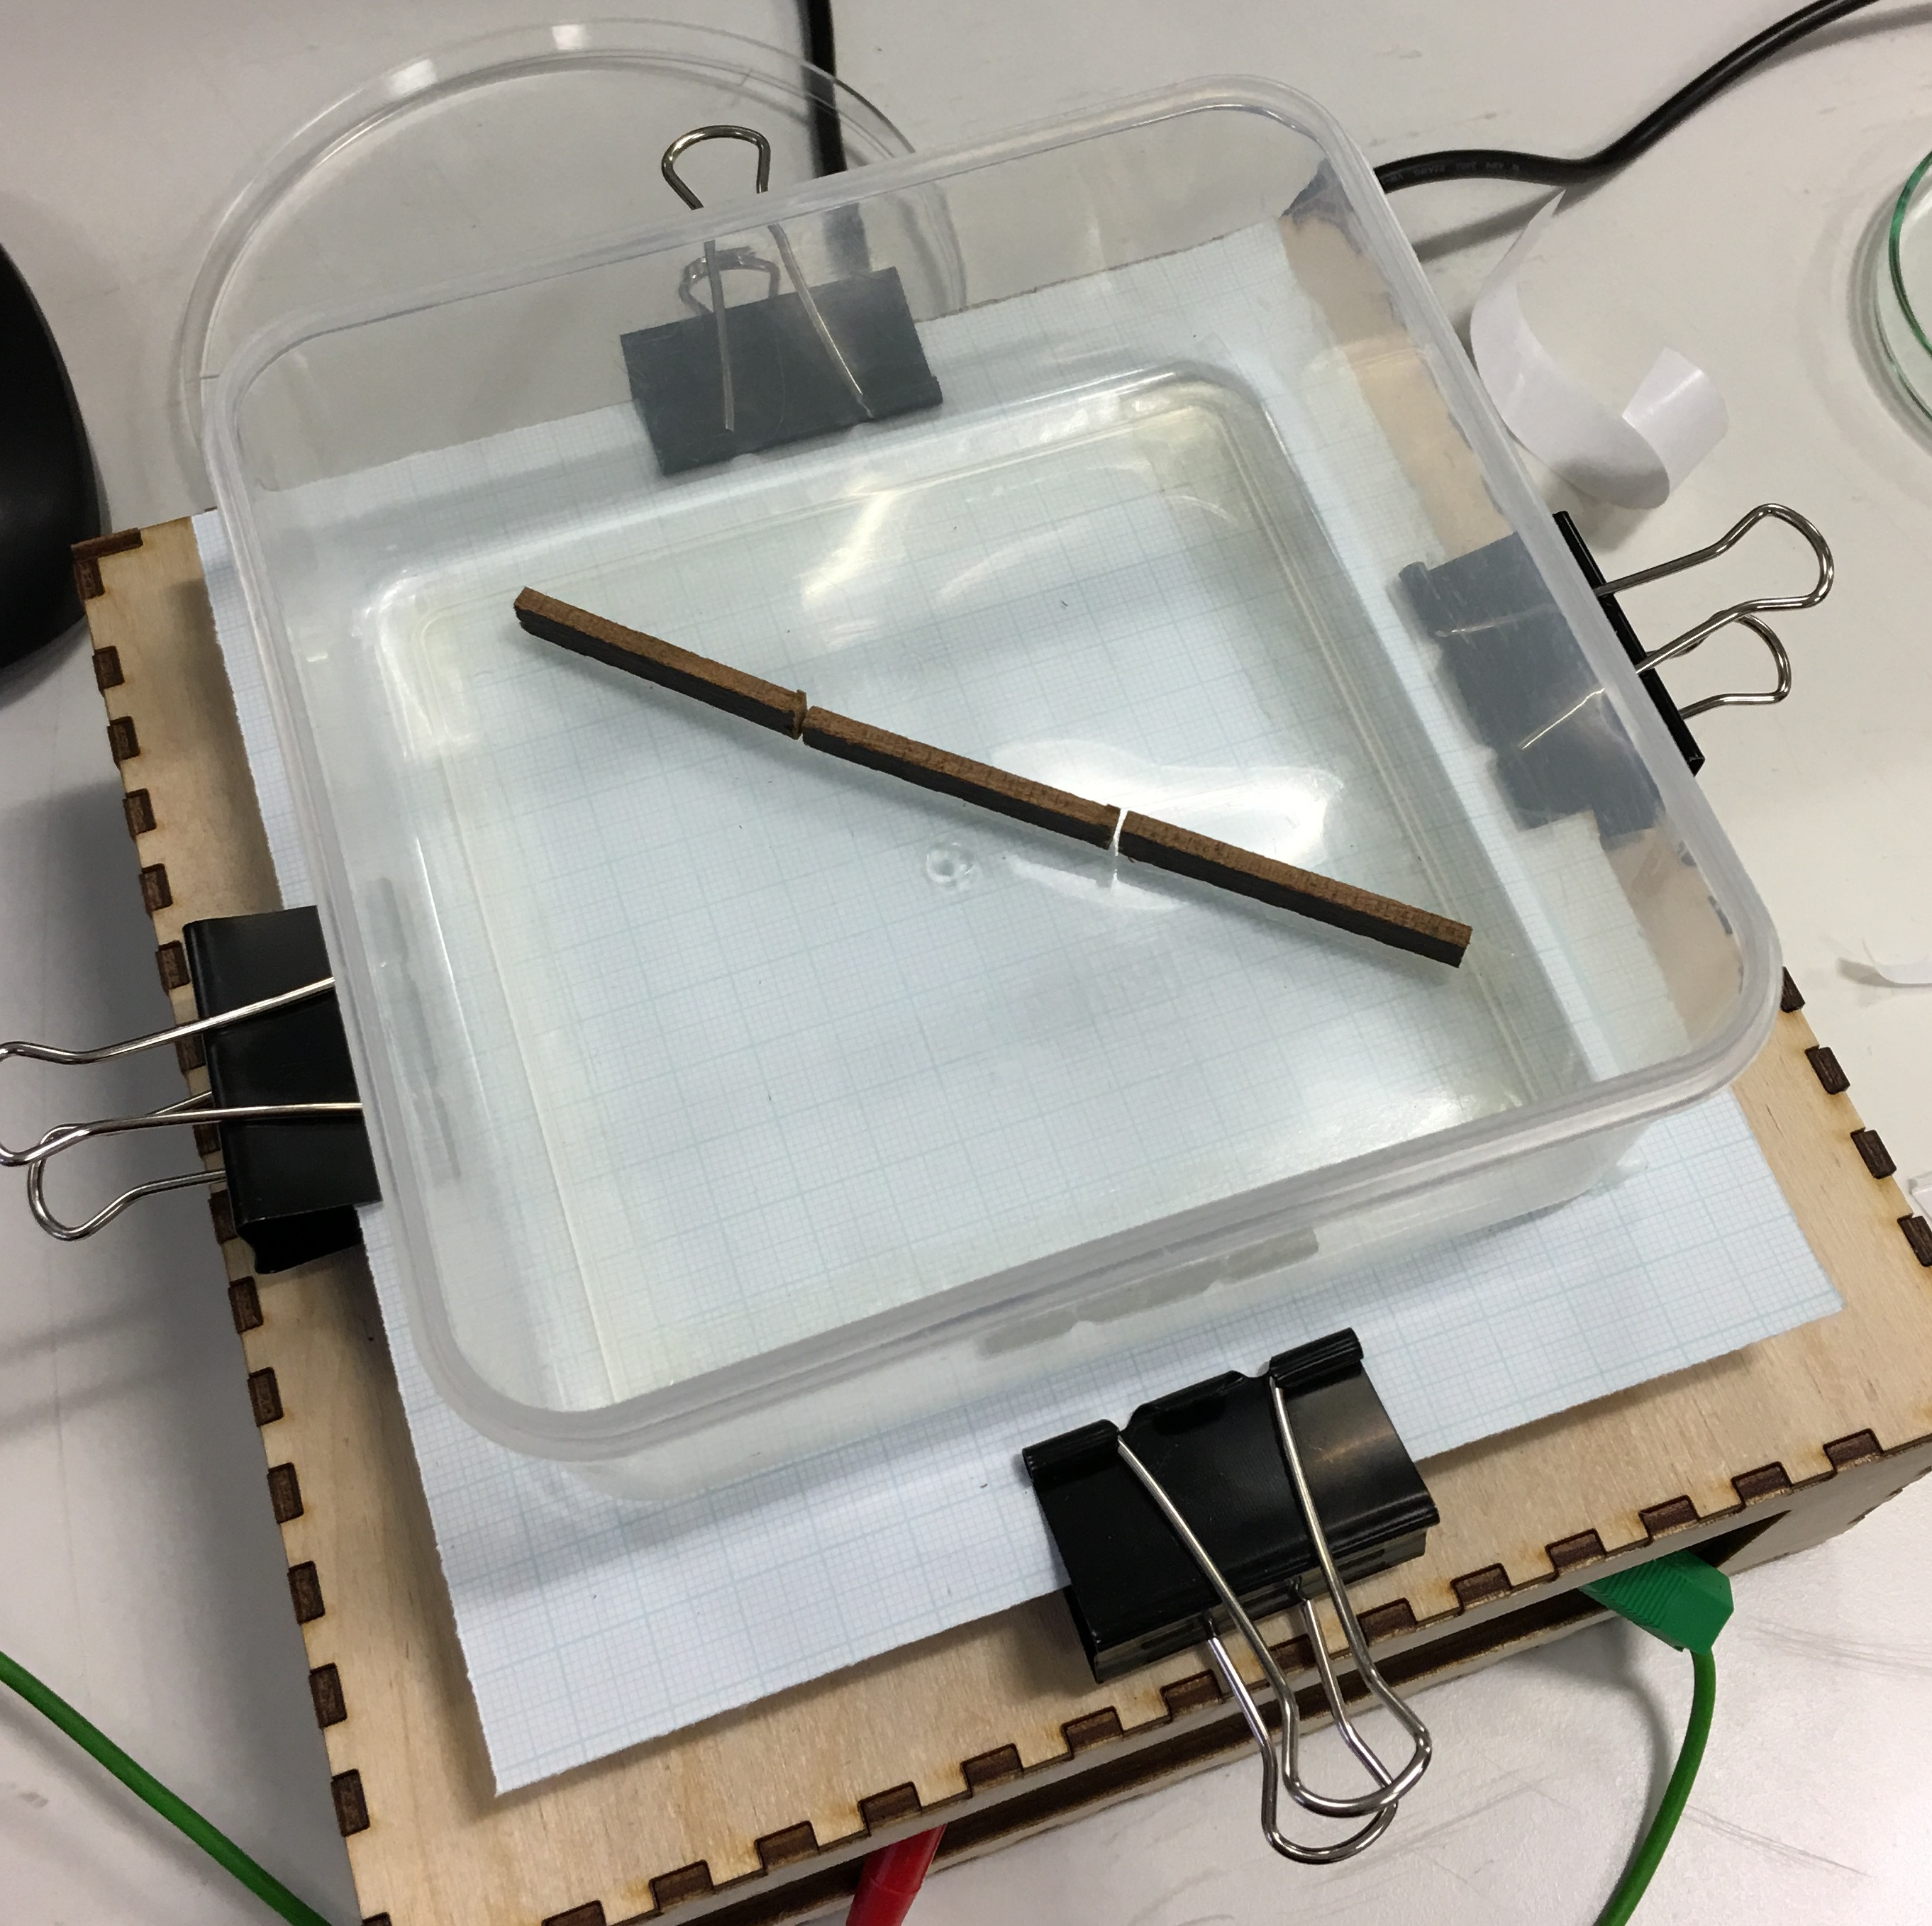
\includegraphics[width=\textwidth]{prototype/exp_rep_imgs/double_slit_setup_1.jpg}
        \caption{Double slit diffraction with slits located far from each other.}
    \end{subfigure}
    \begin{subfigure}{0.475\textwidth}
        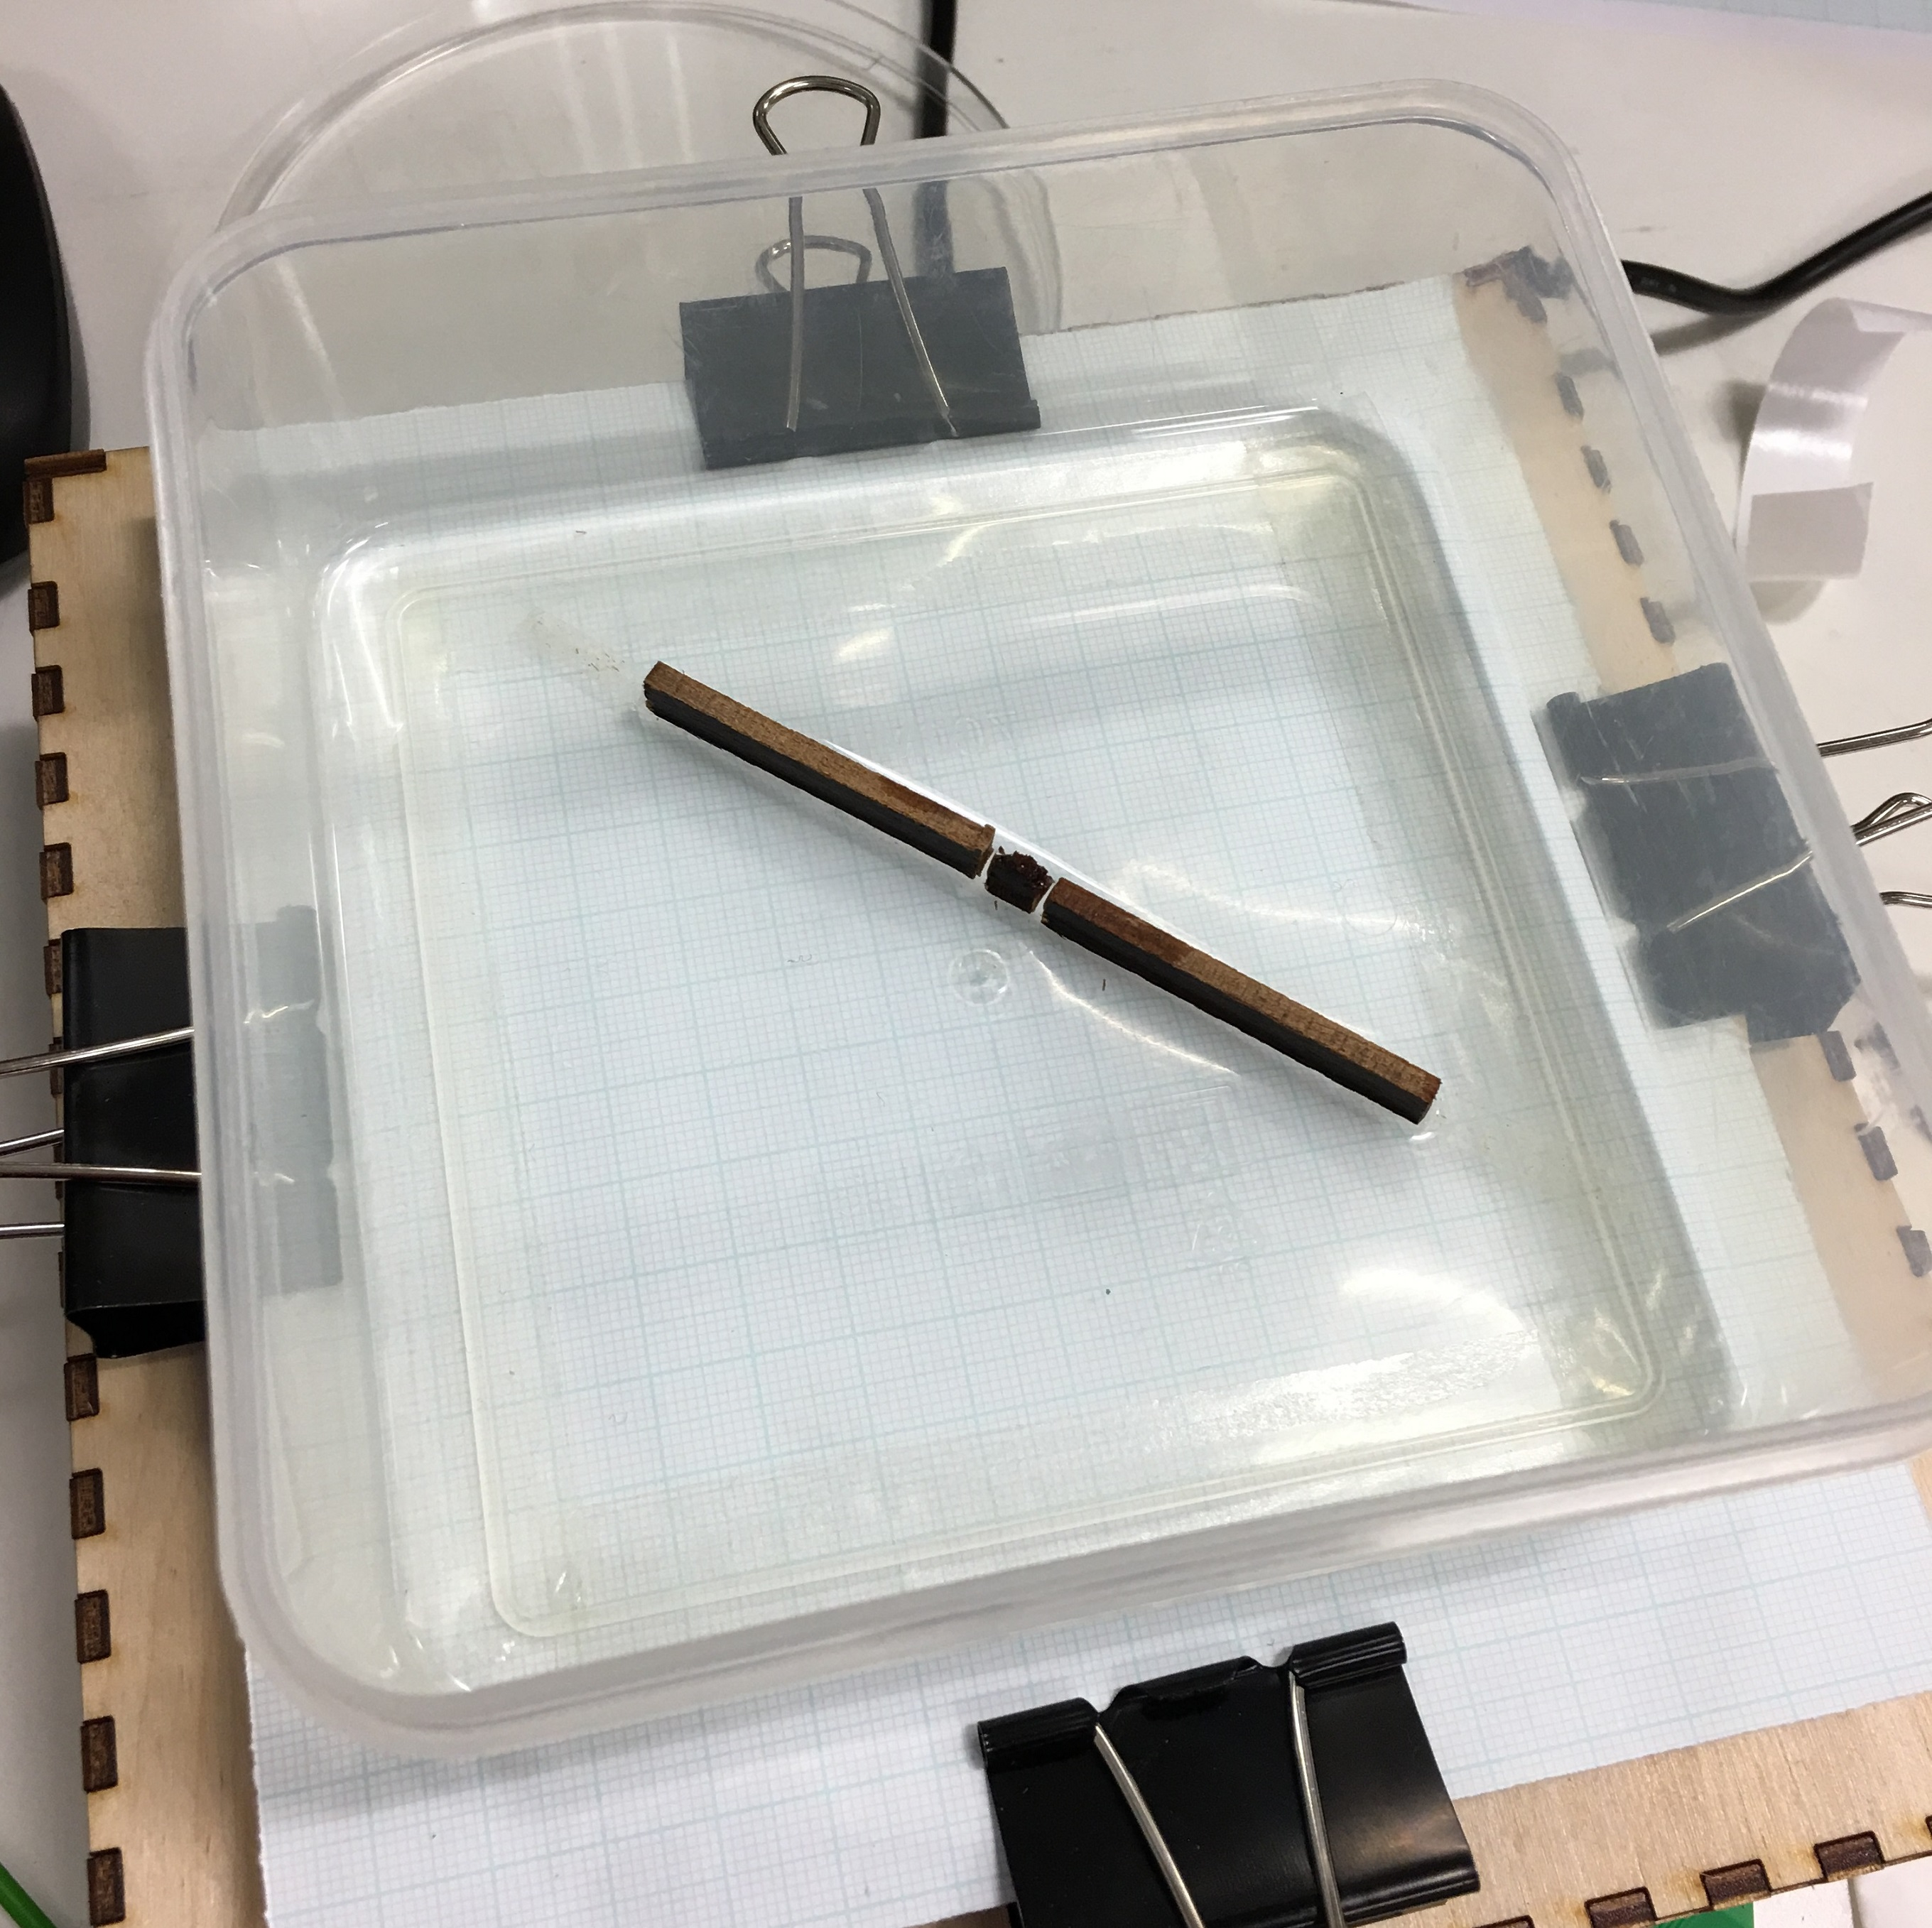
\includegraphics[width=\textwidth]{prototype/exp_rep_imgs/double_slit_setup_2.jpg}
        \caption{Double slit diffraction with both slits located near to each other.}
    \end{subfigure}
\caption{Images of the experimental setup used to try and capture double slit diffraction. A plastic Tupperware box was used in place of a petri dish. }
\label{fig:double_slit_setup}
\end{figure}

By producing droplets and forcing them towards the slits using compressed air, it was found that the silicone oil would crawl up the slit due to surface tension. The tension created a barrier which prevented the droplets from passing through the slit. This led to the use of more extreme methods, such as pushing the droplets with a wooden stick and even tilting the entire box at a large inclination. Both methods proved to be ineffective in overcoming the surface tension.

A proposed solution was to submerge the slits and push the droplets through. No visible diffraction was observed. Eventually the experiment was simplified and reverted to a single slit in a petri dish, where both submerged and non-submerged slits were tested. The same issue with surface tension was encountered, and again no diffraction was observed with the naked eye.

\subsection{Changing Fluid}
With a stable bouncing state achieved, it was decided that a different type of liquid should be tested. This time the experiment was carried out with washing up liquid diluted in water, as research papers have stated that soap water was one of the earliest liquids used to test the pilot-wave theory \cite{protiere2006particle}. It also is a good candidate if the project were to be commercialised or used as an educational tool in schools. The other candidate shortlisted was vegetable oil, as it has a similar viscosity with our previous silicone oil of 50 cSt, but widely available.

The soap water was produced by mixing washing liquid with water and stirring it with a wooden stick. At 50 Hz waves were much more visible due to the green tint from the washing up liquid; it was also predicted that the low viscosity of the liquid would help to produce more stable droplets. At a certain angle, waves produced by the droplets were clearly visible under ambient light.

The Faraday instability regime, a sudden increase in chaotic wave forms on the liquid surface, was also explored. The breaking of the surface also created chaotic motion of droplets, whereby they undergo irregular movements across the surface. By decreasing the amplitude under the Faraday threshold, the surface became calm again, and the only waves visible were the standing waves formed by the bouncing droplets. This was clearly visualised using the soap water as seen in Figure \ref{fig:faraday_inst_regime}.

\begin{figure}[htb]
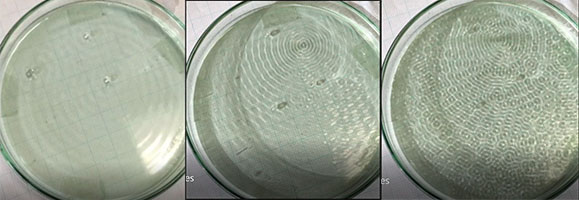
\includegraphics[width=\textwidth]{prototype/exp_rep_imgs/Faraday_inst_regime.jpg}
\centering
\caption{A series of images showing the evolution of a system to the Faraday instability regime, represented with the right-most image. The middle image represents the Faraday threshold, and the leftmost image is the regime where standing waves are formed by bouncing droplets. The diluted soap water produced a green tint.}
\centering
\label{fig:faraday_inst_regime}
\end{figure}

The new liquid also proved to be extremely effective in producing other phenomena that were not possible under silicone oil. Phenomena such as walking and orbiting were also observed and recorded, and Figure \ref{fig:orbit_droplets_interaction} shows an orbiting pair of similar sized droplets. It  was possible to sustain these for around 10 seconds before one is destroyed. Walking can be seen from Figure \ref{fig:double_slit_walking_perimeter}, where a droplet was observed to glide along the edge of the petri dish for many revolutions at a relatively fast speed. In this image, plastic slits were used to test double slit diffraction again. However, surface tension still arose, which motivated a change in technique. The slits were moved towards the droplets instead, the relative motion was thought to produce a similar effect. However, the effects were not visible with the naked eye.

\begin{figure}[htb]
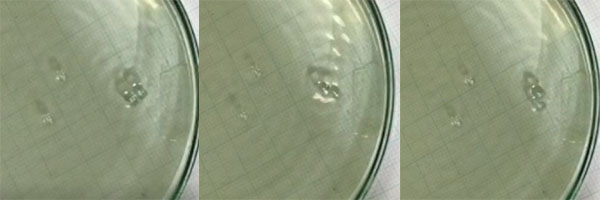
\includegraphics[width=\textwidth]{prototype/exp_rep_imgs/orbit_droplets_interaction.jpg}
\centering
\caption{A series of images showing an orbiting pair of similar sized droplets. Two other bouncing droplets can also be seen in the left.}
\centering
\label{fig:orbit_droplets_interaction}
\end{figure}

\begin{figure}[htb]
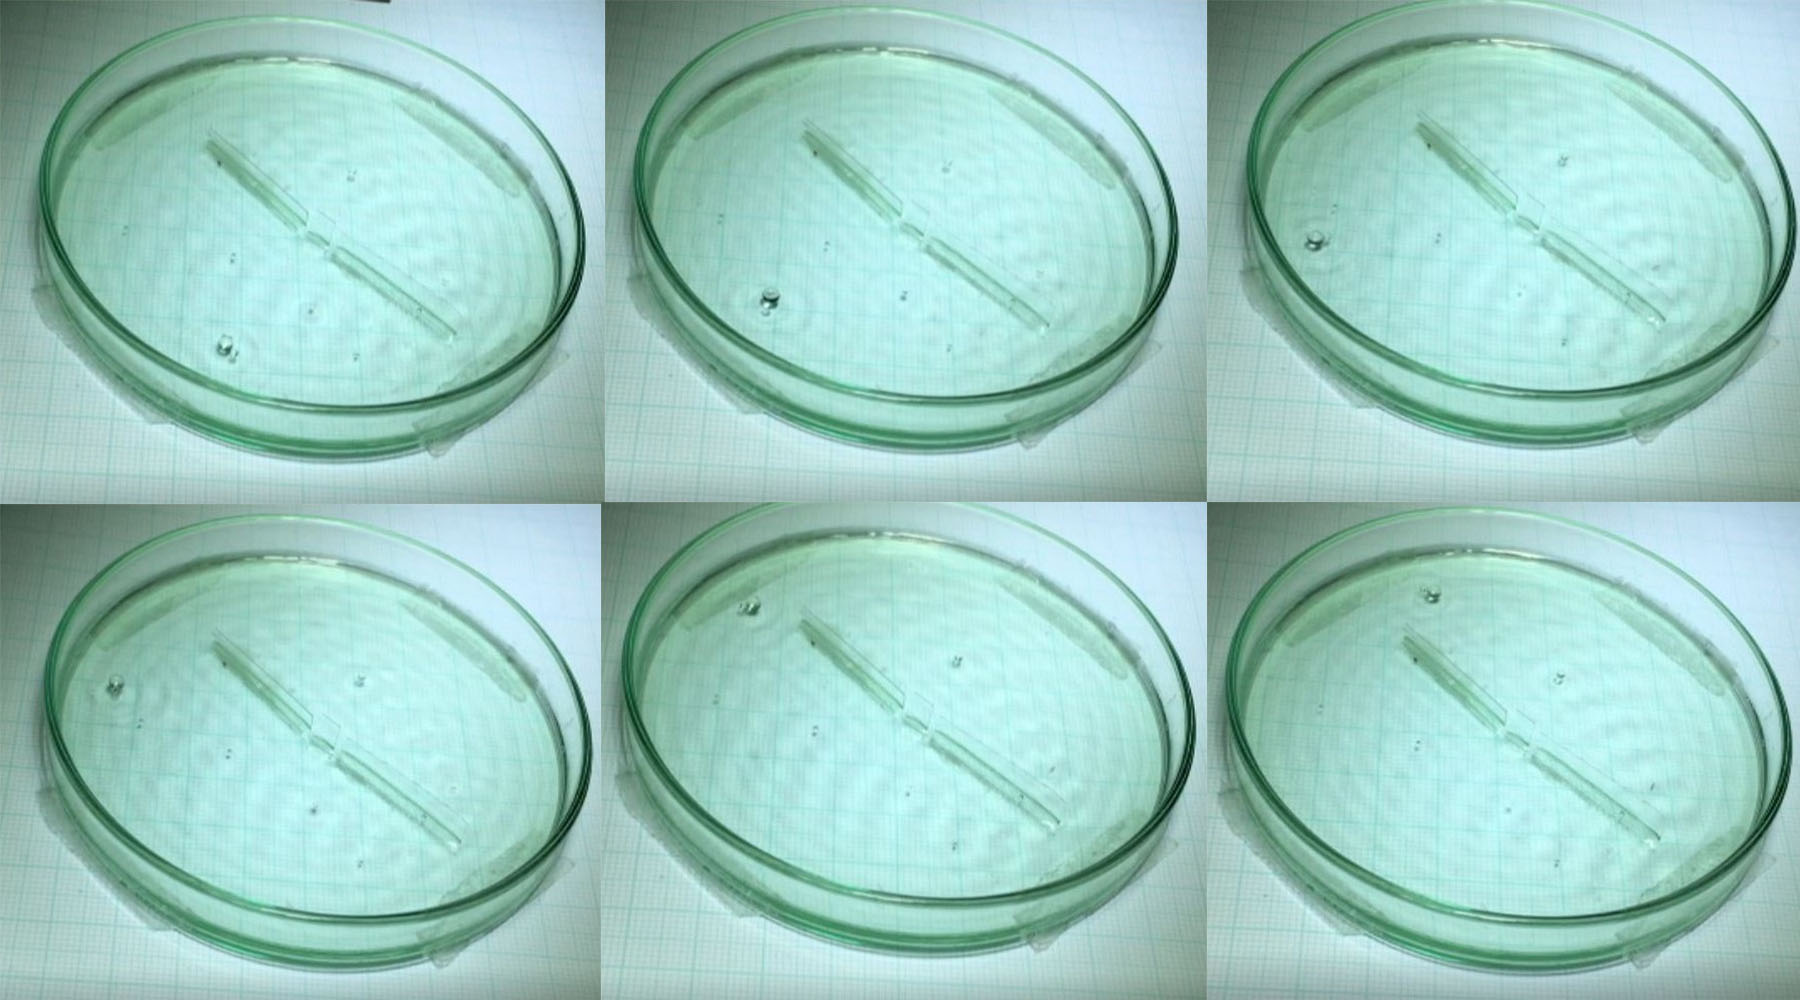
\includegraphics[width=\textwidth]{prototype/exp_rep_imgs/double_slit_walking_perimeter.jpg}
\centering
\caption{A series of images displaying the motion of a walking droplet around the perimeter of the petri dish. The droplet was observed to travel for several rounds before coalescing.}
\centering
\label{fig:double_slit_walking_perimeter}
\end{figure}

As a  result of using soap water, more consistent droplets were created and more quantum phenomena were observed. Another observation included a cluster that resembles a crystalline lattice structure, where three droplets formed a triangular lattice as shown in Figure \ref{fig:triangle_structure}. A bigger cluster formed an irregular lattice that can be seen in Figure \ref{fig:irregular_structure}.

\begin{figure}[ht]
    \begin{subfigure}[t]{0.5\textwidth}
        \centering
        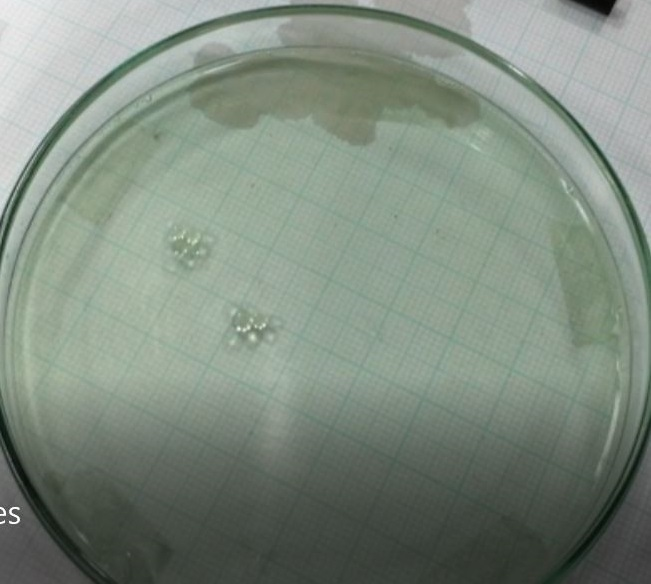
\includegraphics[width=\textwidth]{prototype/exp_rep_imgs/triangular_lattice.jpg}
        \caption{An aggregate of three droplets, formed from the self-assembly of steady state bouncers into a cluster}
        \label{fig:triangle_structure}
    \end{subfigure}
    \begin{subfigure}[t]{0.5\textwidth}
        \centering
        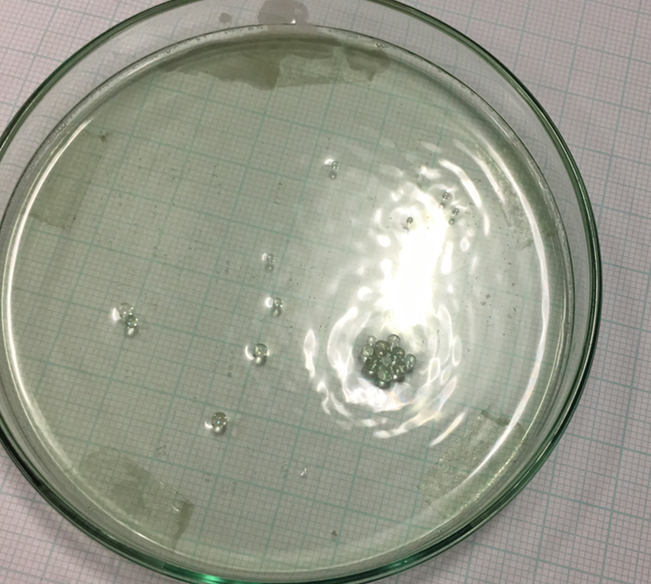
\includegraphics[width=\textwidth]{prototype/exp_rep_imgs/lattice_cluster.jpg}
        \caption{A larger cluster of droplets. They did not form a regular crystalline lattice structure, rather a random assembly. It was observed that droplets would tend towards each other regardless of their initial starting position}
        \label{fig:irregular_structure}
    \end{subfigure}
\caption{Crystalline lattice structures formed by steady state bouncing droplets.}
\label{fig:irregular_structure_evolution}
\end{figure}


To wrap up, food colouring was used to try and enhance visualisation. The result can be seen in Figure \ref{fig:red_dye}. A repelling quadruple was observed. This was predicted by how droplets were in anti-phase when they were in the bound state. If they were in phase, the resultant phenomenon would be the orbiting state.

\begin{figure}[ht]
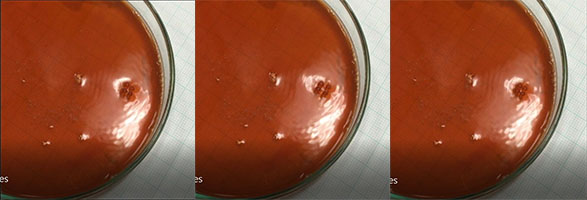
\includegraphics[width=\textwidth]{prototype/exp_rep_imgs/red_dye.jpg}
\centering
\caption{Repelling quadruple droplets with soap water dyed red. This is a much more complex motion due to having four bound droplets. Other than repelling, the droplets were also observed to behave like a viscous liquid.}
\centering
\label{fig:red_dye}
\end{figure}

\subsection{Ultra High Speed Camera}
A high speed camera (Photron Fastcam SA1.1) with the capability to record up to 675,000 fps was rented from the Department of Chemical Engineering, supervised by Dr. Han Wu. This was accompanied with a pair of table-attachable high power  lights, a regular camera for recording at a normal rate (25 fps), a diffuser, and a laptop with the software required to operate the high speed camera. It was discovered that the camera can only record in black and white.

An issue arose when attempting to find the best angle and distance for the camera to have the best focus; positioning the spotlight and adjusting the aperture were necessary to better visualise the final image on the computer.

In this attempt, plastic slits were superglued to the petri dish to attempt diffraction with soap water, although it was uncertain how the glue would have mixed with the soap. The slits are shown in Figure \ref{fig:plastic_slits}.

\begin{figure}[htb]
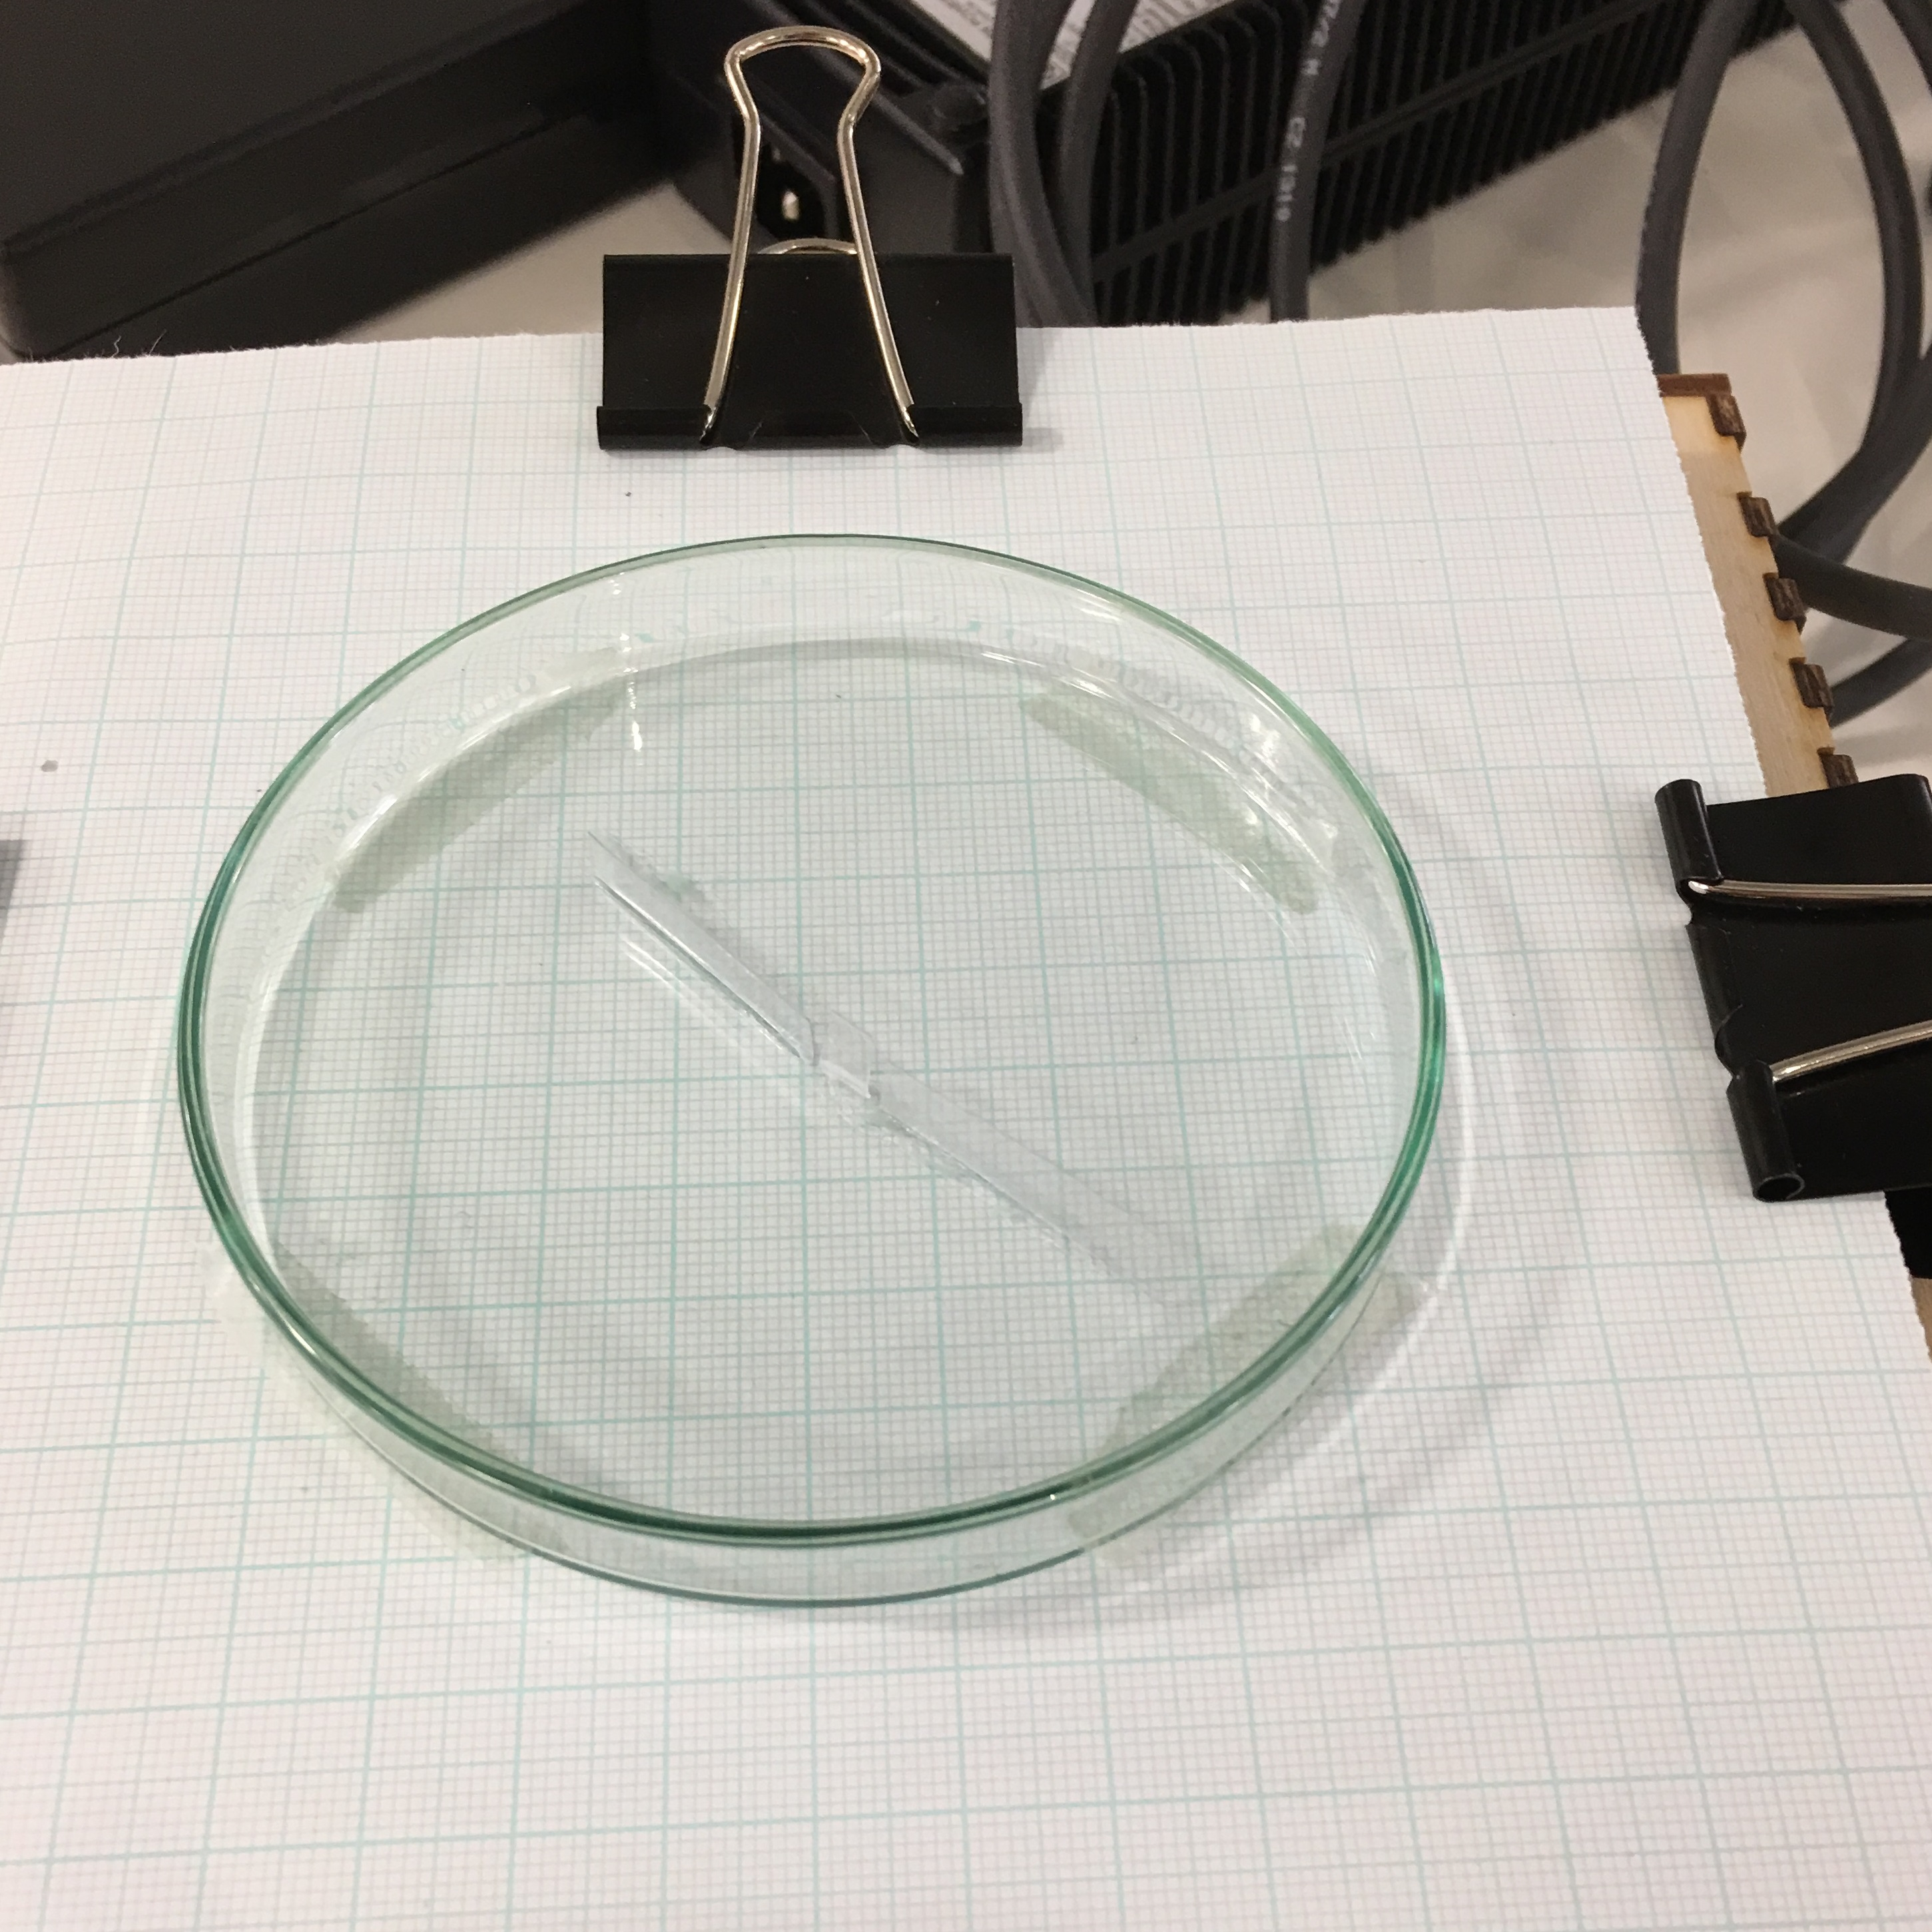
\includegraphics[width=0.5\textwidth]{prototype/exp_rep_imgs/plastic_slits.jpg}
\centering
\caption{Plastic slits were superglued onto the petri dish to form a diffraction grating. This was thought to have a lower surface tension than wood gratings due to the reduced thickness.}
\centering
\label{fig:plastic_slits}
\end{figure}

Initially the frame rate was set to 1000 fps with a resolution of 1024 x1024, giving a video time of around 8 s. A trade-off had to be made between resolution and maximum frame rate, as the highest frame rate at this resolution is 5400 fps. If a higher frame rate was required, the resulting video would have a lower resolution. The trigger was controlled on the computer, and other calibrations were also carried out with the software interface. The setup can be seen in Figures \ref{fig:closeup_highspeedcamera} and \ref{fig:software_highspeedcamera}. The amount of light captured by the lens could also be adjusted, but was usually set to the highest setting, although it was found that lowering this could help with visualisation, since the region was well illuminated due to the presence of the two high-powered lights. In high-speed mode, bouncing and walking were captured. There was difficulty in producing other phenomena, this due to the limited region that was focused on. Sometimes the droplets had to be forced into focus, and this often caused them to break.

\begin{figure}[ht]
    \begin{subfigure}[t]{0.475\textwidth}
        \centering
        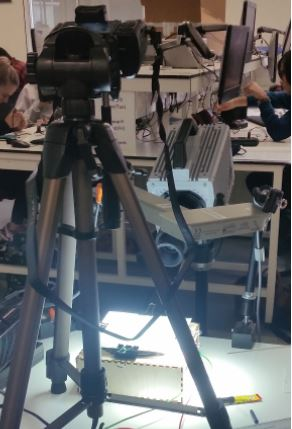
\includegraphics[width=\textwidth]{prototype/exp_rep_imgs/closeup_highspeedcamera.jpg}
        \caption{Closeup on the focusing angle of the high speed camera. Another professional camera was also used to take still images.}
        \label{fig:closeup_highspeedcamera}
    \end{subfigure}
    \begin{subfigure}[t]{0.475\textwidth}
        \centering
        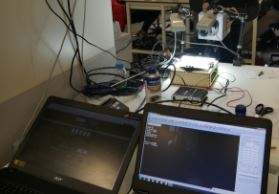
\includegraphics[width=\textwidth]{prototype/exp_rep_imgs/software_highspeedcamera.jpg}
        \caption{Laptops with online function generator and the Photron software, PFV Ver.3681.}
        \label{fig:software_highspeedcamera}
    \end{subfigure}
\caption{Setting up of the high speed camera Photron Fastcam SA1.1, accompanied with high intensity lights and software system}
\label{fig:highspeed_setup}
\end{figure}

Remarkable results were captured with the high speed camera which are summarised and displayed as follows:
\begin{enumerate}
\item  Individual wave fronts were clearly visible, as seen in Figure \ref{fig:highspeed_wave}.
\item  Attempts were made to observe the interference of droplet waves with slit, and to continuously create waves and observe their interaction with  the slits.
\item  Multiple droplets were produced and their interactions with each  other and with the surface are displayed in Figure \ref{fig:highspeed_multiple}.
\item  The Faraday instability regime at high speed is displayed in  Figure \ref{fig:highspeed_faraday}.
\end{enumerate}

\begin{figure}[htb]
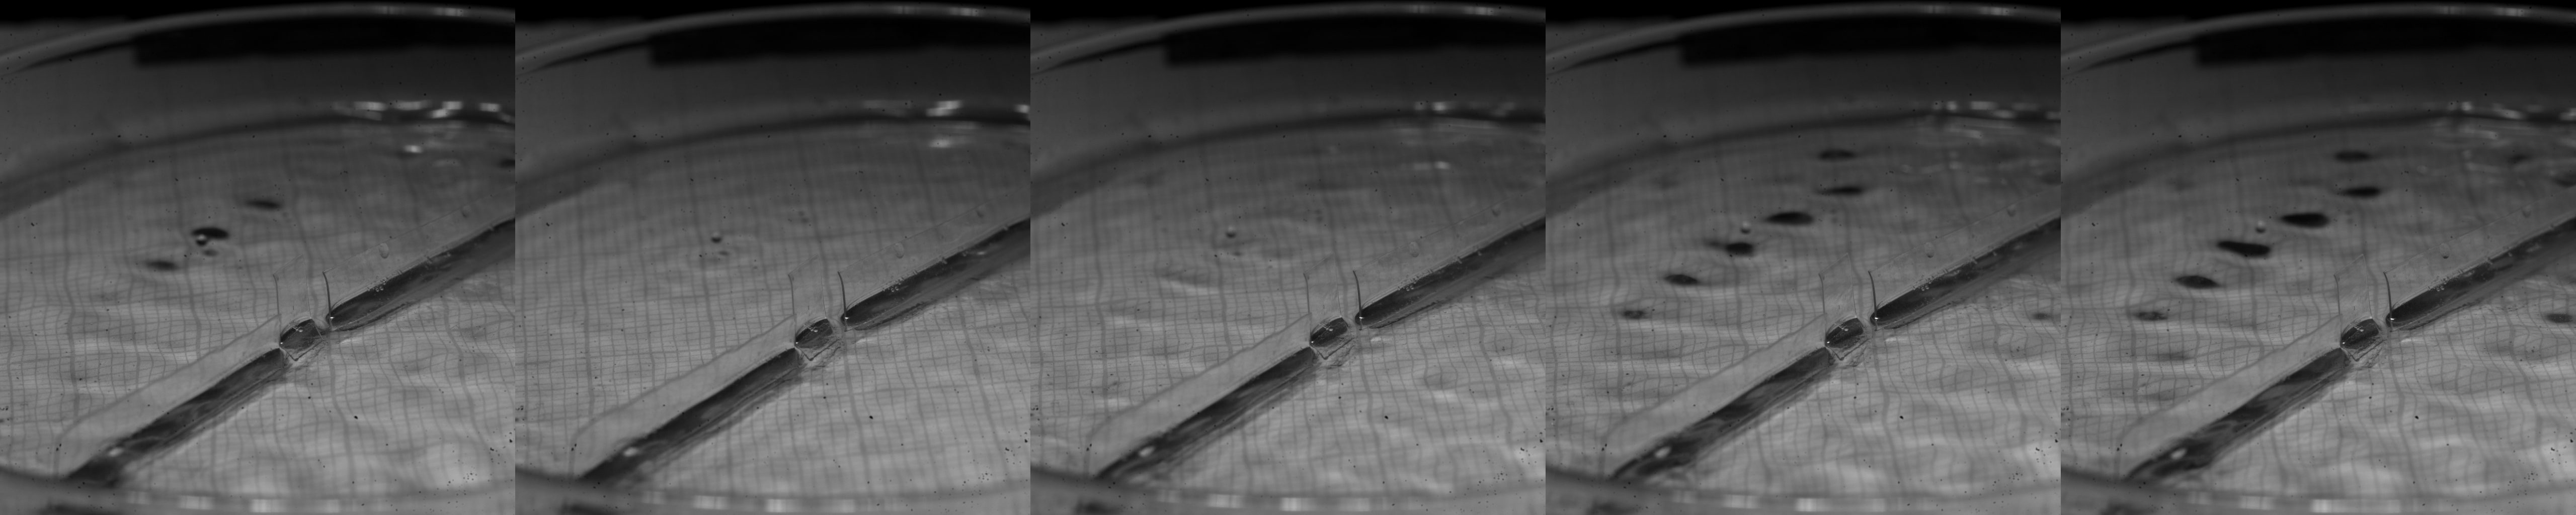
\includegraphics[width=\textwidth]{prototype/exp_rep_imgs/highspeed_wave.jpg}
\centering
\caption{Single droplet standing wave recorded at 1000 fps, series is composed of images taken at every 5 frames.}
\centering
\label{fig:highspeed_wave}
\end{figure}

\begin{figure}[htb]
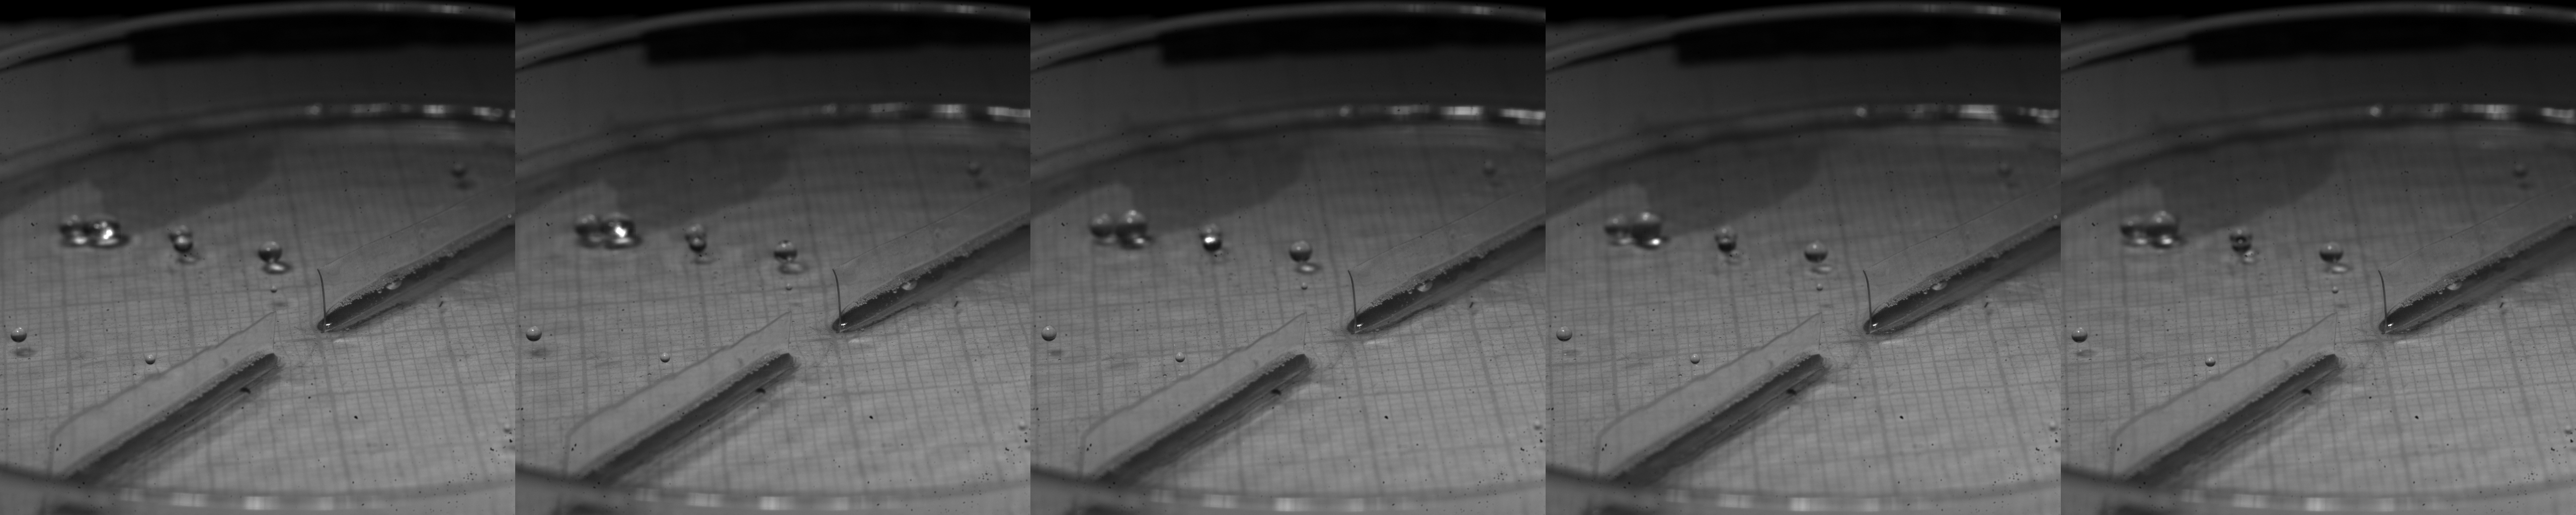
\includegraphics[width=\textwidth]{prototype/exp_rep_imgs/highspeed_multiple.jpg}
\centering
\caption{Multiple droplets displaying standing waves and bound states recorded at 1000 fps, series is composed of images taken at every 5 frames.}
\centering
\label{fig:highspeed_multiple}
\end{figure}

\begin{figure}[htb]
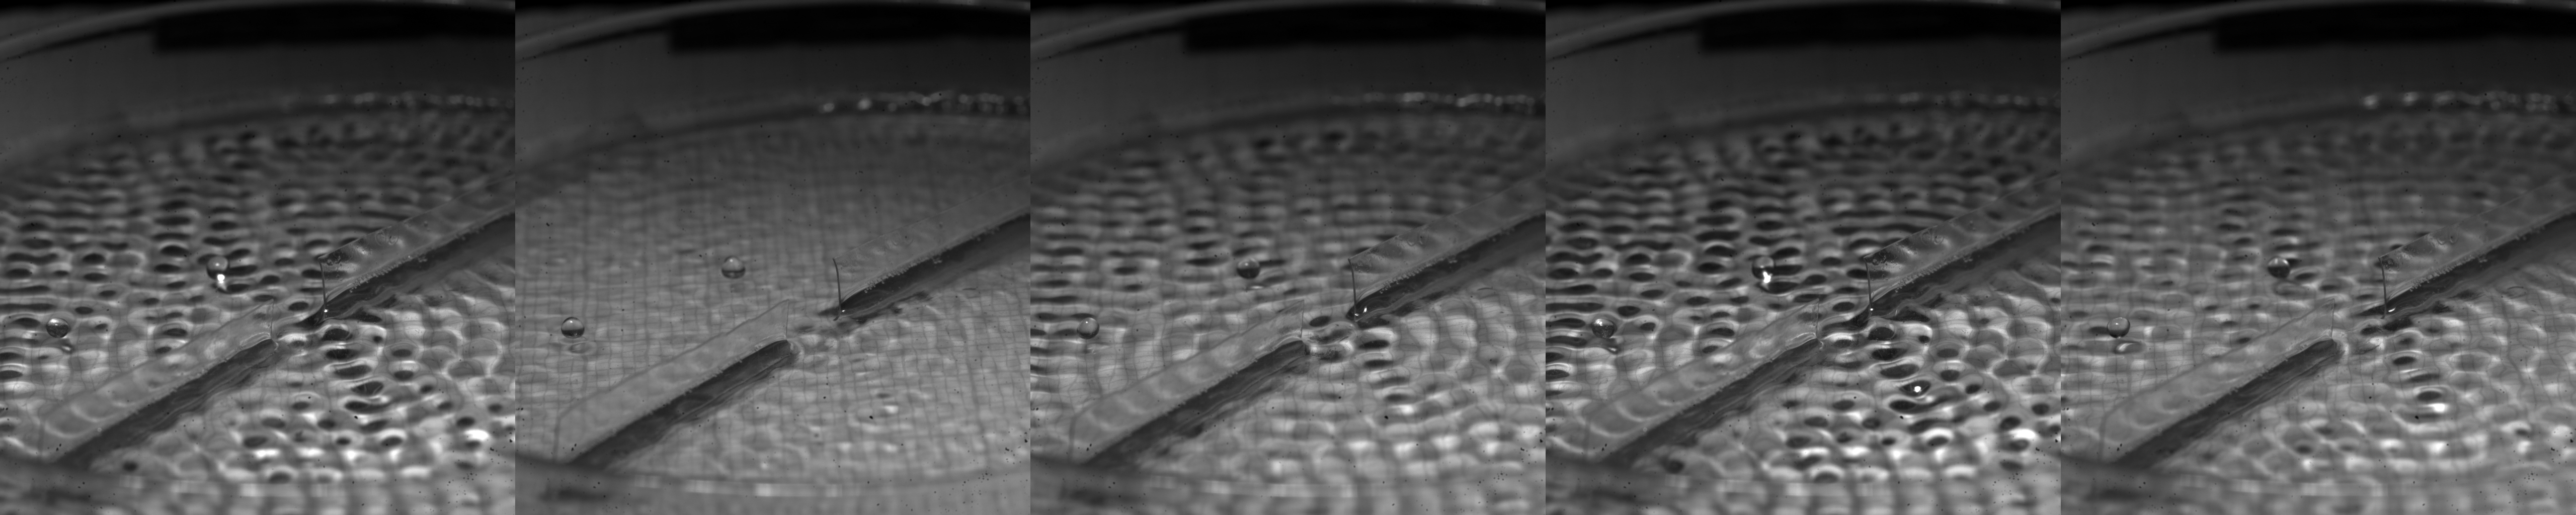
\includegraphics[width=\textwidth]{prototype/exp_rep_imgs/highspeed_faraday.jpg}
\centering
\caption{The surface of the soap water under the Faraday instability regime, recorded at 1000 fps, series is composed of images taken at every 5 frames.}
\centering
\label{fig:highspeed_faraday}
\end{figure}

Motion tracking was postulated to be able to track the high speed footage at a high level of accuracy. This was carried out in Adobe AfterEffects, where the tracking results are illustrated in Figure \ref{fig:tracking_droplet}.

\begin{figure}[htb]
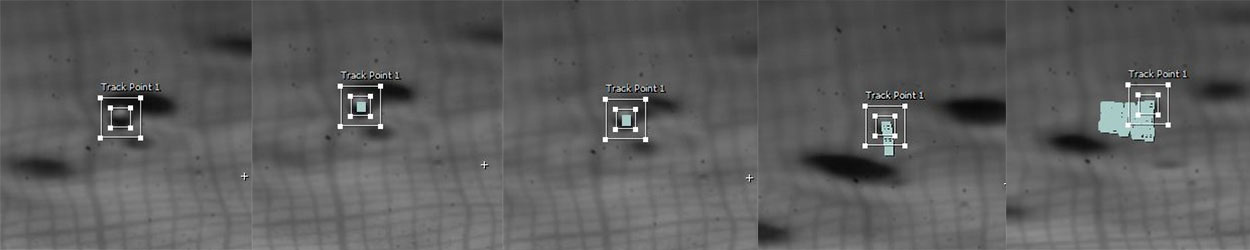
\includegraphics[width=\textwidth]{prototype/exp_rep_imgs/tracking_droplet.jpg}
\centering
\caption{Motion tracking carried out on Adobe AfterEffects, the buildup of white dots represent the path of the droplet in the form of coordinates.}
\centering
\label{fig:tracking_droplet}
\end{figure}

By applying motion analysis to a null object created in AfterEffects,  a sequence of time frames was created as shown in Figure \ref{fig:after_effects_interface}. The time frames were copied into a text document and imported into Microsoft Excel.

\begin{figure}[htb]
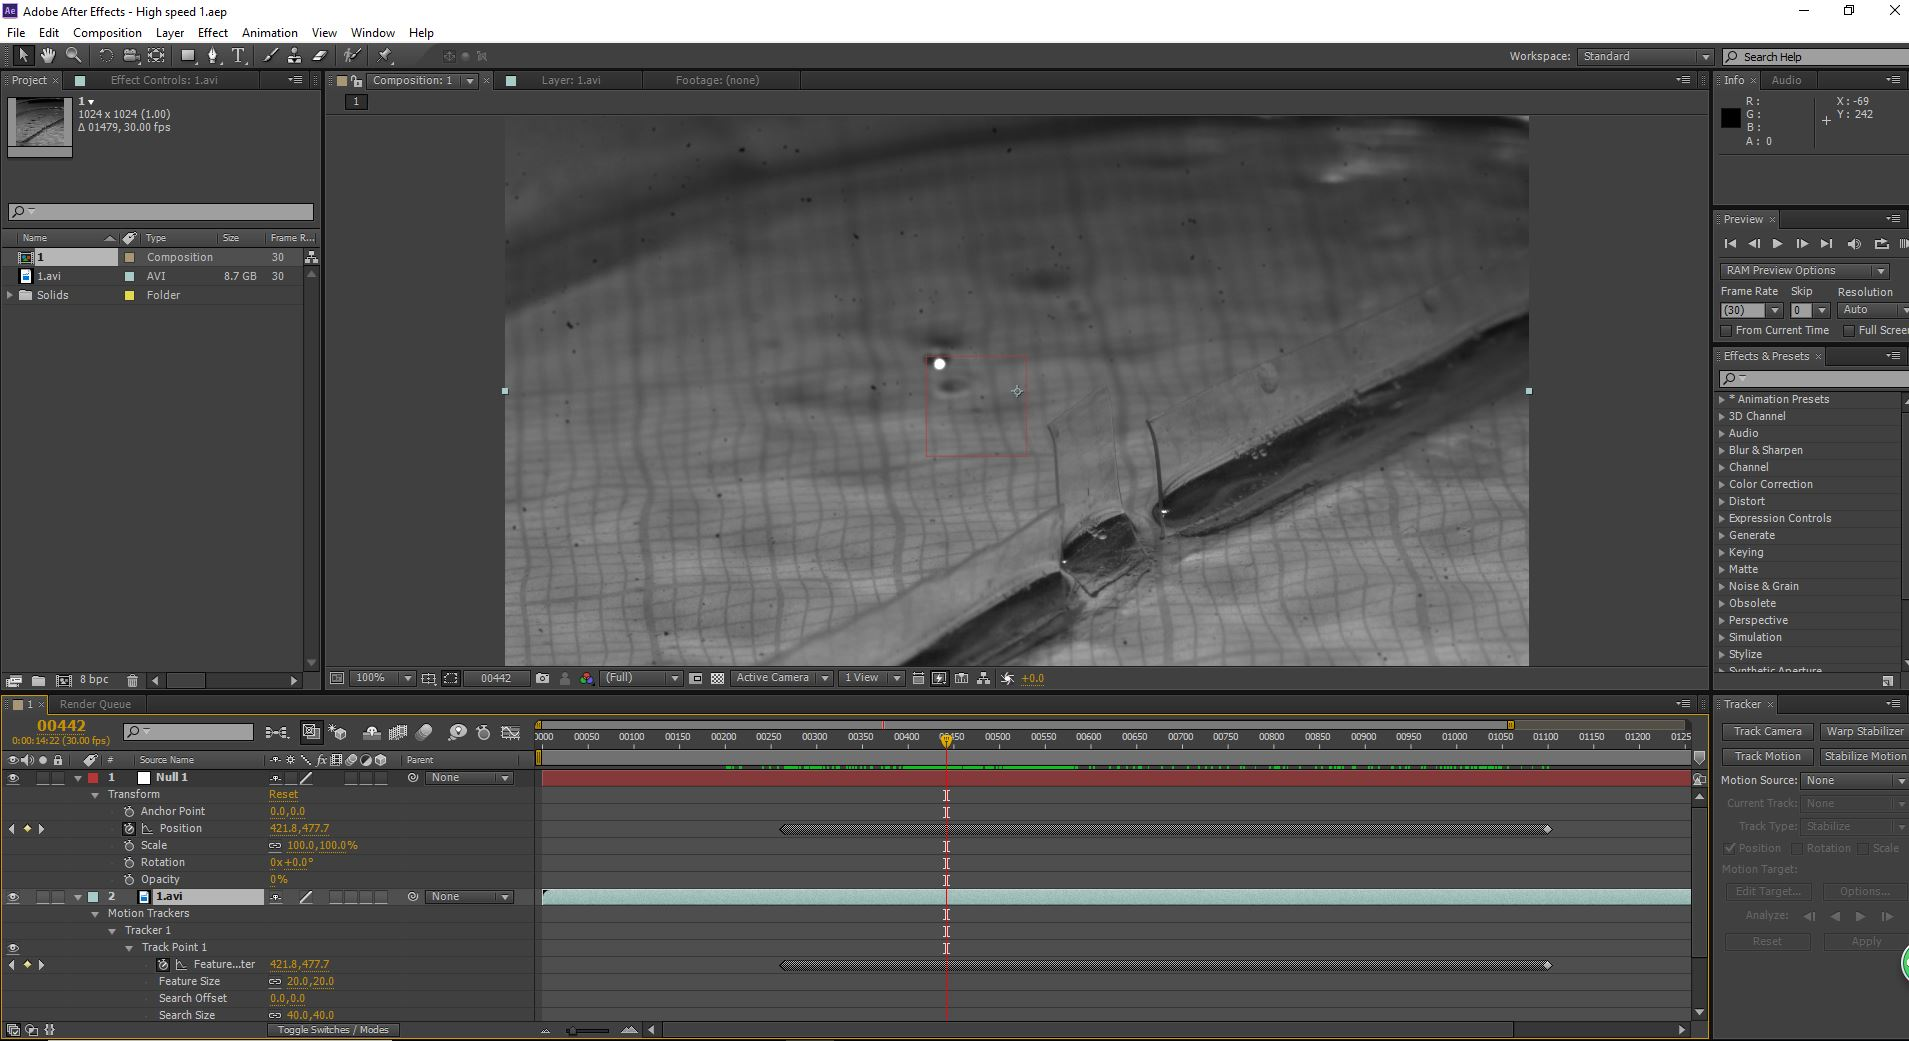
\includegraphics[width=\textwidth]{prototype/exp_rep_imgs/after_effects_interface}
\centering
\caption{A screen-shot of Adobe AfterEffects interface after tracking had been analysed. Key frames are clearly visible on the timeline where they have been applied onto the null object}
\centering
\label{fig:after_effects_interface}
\end{figure}

The exported coordinates were of the format: frame, x coordinates, y coordinates. The coordinates were given in units of pixels. Since the video was recorded at 1000 fps, each frame corresponds to 1 ms. The y coordinates were plotted as a function of time, as shown in Figure \ref{fig:droplet_amplitude_graph}. Converting to time units allowed for a clearer representation of the time scale of bounces.

\begin{figure}[htb]
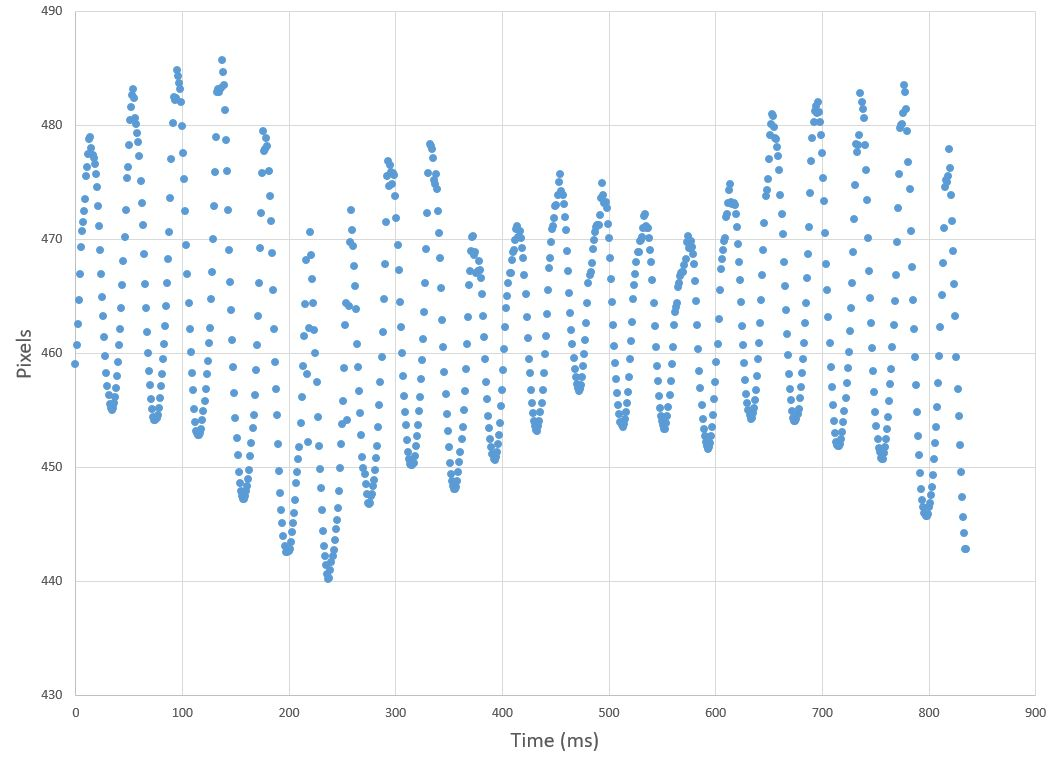
\includegraphics[width=\textwidth]{prototype/exp_rep_imgs/droplet_amplitude_graph.jpg}
\centering
\caption{The y coordinates of the bouncing droplet as a function of time. Oscillatory motion can be seen, and the period is roughly constant.}
\centering
\label{fig:droplet_amplitude_graph}
\end{figure}

Inferences can be drawn from this graph. First of all, the y coordinates do not strictly represent the height of each bounce. This is because the camera is not aligned with the surface of the liquid, but at an angle, due to limitations in focusing and capturing sufficient light. However the main contribution to the y coordinates is the change in height, so the graph clearly demonstrates an oscillatory motion of constant period. Difficulties in determining a quantitative measure of height arose due to the y coordinates being a relative measure. A control needs to be set in order to quantify the y coordinates in units of length. For example, knowing the exact length of an object that is captured by the high speed camera. This allows for a comparison between length and resolution.

A rough estimate of height could be carried out since the diameter of the petri dish was known. The plastic grating is somewhat centred on the diameter of the petri dish. Using Figure \ref{fig:plastic_slits}, the centre of the petri dish can be estimated to be on the right edge of the centre grating. Drawing a straight line upwards to the edge of the petri dish gives an estimate of the radius which is known to be 5.08 cm. The resolution of the video was known, as it was set on the high speed camera to be 1024x1024. The distance to the edge was measured to be about 430 pixels. This means that the length conversion is 0.118 mm per pixel. Typical amplitudes from Fig. 30 are about the size of 15 pixels, which gives a height close to 1.8 mm. This is overestimated as the video was captured at angle of around 30 degrees as seen in Figure \ref{fig:closeup_highspeedcamera}. This stretches out the actual length, and can be compensated for by multiplying by the sine of the angle, which gives around 0.9 mm.  

From Figure \ref{fig:after_effects_interface} it can be seen that there is a bright dot at the bottom of the droplet. This was found during the review of the entire high speed video. During some of the bounces, it seems that a bright beam of light was produced. A frame by frame investigation of this phenomenon was conducted. This can be seen in Figure \ref{fig:strange_light} where a droplet completes a bounce.

\begin{figure}[htb]
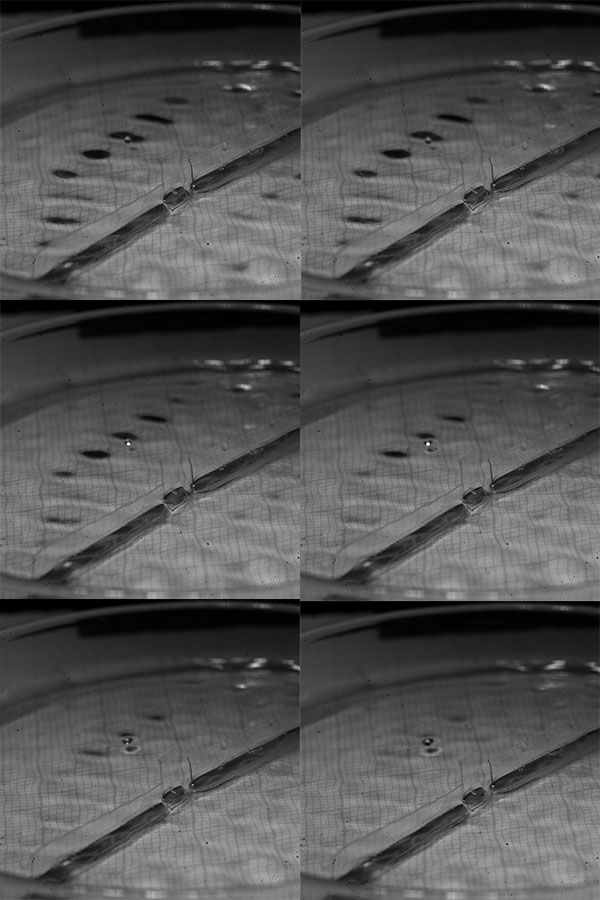
\includegraphics[width=0.8\textwidth]{prototype/exp_rep_imgs/strange_light.jpg}
\centering
\caption{A frame by frame capture of the droplet motion and the formation of standing waves. In the middle two images a white dot can be seen for a few of the bounces.}
\centering
\label{fig:strange_light}
\end{figure}

This was an unexpected result. Close inspection of the high speed video gives interesting qualitative results. Certain bounces are actually two consecutive bounces with the first having a very small amplitude. Bounces that produce a beam of light are single bounces and seemed to propel to a greater amplitude. This suggests some sort of momentum conservation. Light beams also seem to occur from consecutive bounces. The droplet also seems to produce larger wave ripples as it hits the liquid surface. It is hypothesised that at certain oscillations, the droplet has built up enough potential energy to produce more energetic waves and even light. From Fig. 31, it also can be seen that the beam of light existed for longer than 1 ms since this is a frame by frame representation and the video was captured at 1000 fps. This means that it cannot be a single photon. A cascade of photons is required to capture a prolonged period and large cross section, which acts like a laser. There has been research conducted that suggested the possibility of droplets demonstrating atomic electron cloud density under the Faraday regime \cite{oza2013trajectory}.

Further investigation was done in trying to figure out the cause of horizontal motion under the bouncing regime. This was not visible using the naked eye, which is why it remained unknown until now. A possible explanation lies in the use of the plywood plate and foldback clips. There could be random impulses due to the transmission process through the plate. The transmission of waves through a different material is much more complex, and could have resulted in a modified driving force. The sinusoidal waveform could interact with itself in the wood and superimpose to produce another waveform, which can also explain why the amplitude is not constant.

The horizontal impulse is due to the droplet colliding with the side of the bulge, as explained in \ref{theory}. The inclined surface can further complicate the propagation of light. The high intensity light was positioned such that it is almost normal to the surface of the liquid. A portion of it will transmit into the liquid, while others reflect on the surface. The transmitted intensity can further reflect off the bottom of the petri dish or transmit through. The bulge of the wave can act as a medium that focuses light and sends through a coherent beam under certain conditions.

\subsection{Improvements and Considerations}
The table-top demonstration has shown to be effective in producing various droplet behaviours that were predicted by theory. It has fallen short in trying to test diffraction phenomenon or producing more quantitative results, but the progress has been very promising given the time frame and budget. To motivate further investigation, improvements and considerations have been proposed which will be discussed.

\subsubsection{Branding}
The team wants to give the device a distinct branding to show its identity, if it were to be commercialised. Possible considerations include painting the plywood box and printing a ``UCL'' logo. There have been unique and creative methods adopted, such as using foldback clips as clamps or graph paper as a grid. These methods were chosen such that they are extremely reproducible by anyone with a basic knowledge of the setup. This is something that the team wanted to show: a device that is cost-effective, yet very attractive, which is why giving an identity is seen to be very important.

\subsubsection{Improving the plywood box}
In this project, the height of the plywood box was slightly too short, such that plywood finger joints had to be inserted into the gap below the loudspeaker to secure it. One solution will be to laser-cut a new box with the corrected dimensions. However, a more cost-effective method would be to cut circular plywood rings to replace the finger joints, which would fit perfectly in the gap, as the loudspeaker is circular itself. The circular ring would also be more reliable, as it is regularly shaped and provides better support at all angles.

\subsubsection{Rotating liquid bath}
An additional centripetal acceleration would be applied through a rotating bath. The petri dish would therefore experience a vertical force from the loudspeaker, superimposed with a central force that acts towards the centre of the petri dish. This could cause droplets to be forced toward the centre.

Depending on the speed of the rotation, it may not cause the droplets to move in the direction of the centripetal acceleration. There is always a degree of restoring force due to surface tension which has to be overcome. This provides a measure of restoring force since the centripetal force can be calculated using \ref{equ:centripetal_force}:
\begin{equation}
F_c = \frac{mv^2}{r} = m \omega^2 r 
\label{equ:centripetal_force}
\end{equation}

For two droplets that are 'repelling' this will create the illusion that they are orbiting each other

\subsubsection{Observing a double slit interference pattern}
This experiment has demonstrated, enough phenomena (`bouncing', `walking', `orbiting', surpassing of Faraday regime etc.) to provide evidence for the Pilot-Wave theory, which opposes the Copenhagen interpretation of quantum mechanics. With this, double slit interference should be observable provided that enough droplets travel through the slits and their end position is recorded. It was thought that a high speed camera should be able to capture the wave's interaction at the slit, and how two waves interfere with one another at close range.

\subsubsection{Observing quantum tunnelling}
Quantum tunnelling was observed by another research group \cite{brady2014bouncing} whereby there is a barrier at the edge of the petri dish, and a body of fluid on the other side also driven at the same frequency. It was shown that on rare occasions the droplet was able to pass through the finite width barrier and end up on the other side. This result proves the possibility of observing quantum tunnelling, a purely quantum phenomenon, at a macroscopic scale.

\subsubsection{Improvements on motion tracking}
It has been demonstrated that the droplets follow irregular motion within the Faraday regime. By recording the droplet motion for a prolonged period of time, it could be shown that the resultant path has high levels of similarities to the atomic electron cloud density. 

This is likely to be feasible with the current setup and software. A proper top-down video needs to be captured in order to eliminate parallax and scaling errors. The difficulty would lie in the tracking process, as the chaotic surface hinders the tracker's ability to follow the droplet. However, the video can be broken down into shorter pieces, where each piece is tracked individually. By reconstructing the entire path through plotting the time frame coordinates, a similar pattern should be found.

\subsubsection{Method of producing droplets}
A common issue faced was producing droplets of consistent size. Multiple mechanisms were thought of, including a spring loaded pinpoint which would oscillate vertically and constantly dip into the fluid and create a droplet.

Another proposal was for a rotating mechanism which has multiple pinpoints of constant separation on a wheel. Once rotated, each pinpoint would prick the surface and create a droplet. This has the benefit of producing multiple droplets very rapidly and of providing them with horizontal momentum, which could be used to push droplets towards any desired direction. This may be beneficial in testing double slit interference, where droplets need to travel through thin slits.

\subsection{Conclusion}
The pilot-wave theory has been successfully demonstrated through observing bouncing droplets with 50 cSt silicone oil and soap water. Advanced phenomena for bouncing droplets such as walking, orbiting, repelling, crystalline lattice structure and Faraday instability have also been observed and recorded. Soap water was found to be the most effective liquid in generating sustainable droplets, it’s intrinsic colour has helped in better visualise standing waves without the need of spotlights. Further recording at 1000 fps was carried out using a high speed camera. Results exhibited wave formation from the bouncing droplet on the liquid surface, thus clearly demonstrating wave-particle duality. Through motion tracking carried out on Adobe AfterEffects, the amplitude of droplet bounce was measured and found to be oscillatory. Discrepancies arising from inconsistent amplitude and horizontal motion can be attributed to the apparatus’s limitations and parallax arising from the recording angle. Were we afforded more time, we could have tested double slit interaction using created droplet creating mechanisms in order to detect quantum phenomena.
